
This section describes the background estimation methods used in the di-Higgs analysis. 
The simulated event samples summarised in Section~\ref{sec:DiHiggs:simulation}
are used to model all background processes, except for processes with fake-\tauhad\ 
which are estimated using data-driven techniques, as discussed below. 
The \ttbar\ with true-\tauhad\ and Z+HF templates are taken from the MC prediction
but their normalisations are derived from data 
as included as freely floating parameters in the final fit,
as described in Section~\ref{sec:fit}TODO: add reference to fit section. 
Events with electrons or muons that are misidentified as \tauhad\ objects, 
dominantly coming from the \ttbar\ production, 
represent a minor background in the analysis and they are estimated from simulation. 

\subsection{Fake-$\tau$ backgrounds in the \lephad channel}
\label{sec:DiHiggs:lephadfake}

Background events where a jet is misidentified as a \tauhad, 
referred to as fake-\tauhad\ events, 
are estimated using a data-driven method due to imperfect MC modelling of these processes:
the `fake factor' (FF) method.
In short, the FF is the ratio of 
the number of events with fake-\tauhad(s) in one region to another region.
% the number of SR events with a fake-\tauhad,
% to the number of CR events with a fake-\tauhad.
In this analysis, 
the numerator of the FF is the number of fake-\tauhad\ events in the
SR, and the denominator is the number of fake-\tauhad\ events in the dedicated 
anti-\tauhad\ enriched region (anti-\tauhad\ region), provided by the
anti-\tauhad\ selection.
The anti-\tauhad\ selection is defined in detail in Section~\ref{sec:antitau-selection}.
In the formula form, the FF is given as:
\begin{equation}
\mathrm{FF} =  \frac{N(\text{loose }\tauhad)}{N(\mathrm{anti}\mhyphen\tauhad)} 
\end{equation} 
where $N(\text{loose }\tauhad)$ ($N(\mathrm{anti}\mhyphen\tauhad)$) is the number of 
data events with a nominal \tauhad\ (anti-\tauhad) with 
contributions from true \tauhad\ subtracted from each term.
In the case where the event contains more than one anti-\tauhad, 
one is chosen randomly. Derived variables used in the analysis,
such as the \MET, $m^{\mathrm{MMC}}_{\tau\tau}$ and \MET$\phi$ centrality 
are calculated in the same way as for signal events, 
but with the anti-\tauhad\ taking the place of the loose \tauhad\ candidate.

The fake-\tauhad\ can have different origins. 
In Figure~\ref{fig:fakes:feynman}, two Feynman diagrams are shown
for the two dominant processes contributing to the fake-\tauhad\ background,
which are the \ttbar\ and multi-jet (QCD) processes. 
In the \ttbar\ events, the fake-\tauhad\ typically originates from quark initiated jets from 
top-quark decay; in multi-jet events jets initiated from both quark and gluon can be
misidentified as \tauhad. 
\begin{figure}[htbp]
\centering
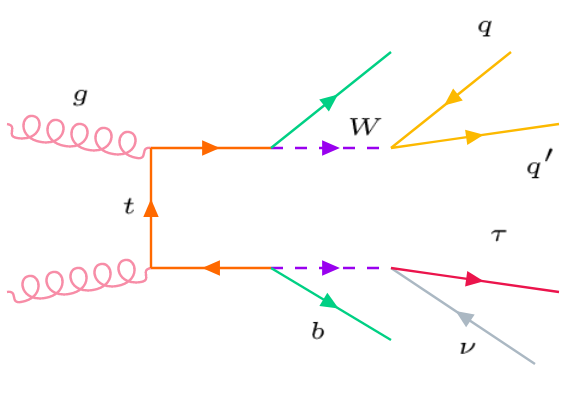
\includegraphics[width=.33\textwidth]{DiHiggs/plots/feynman_ttbarfakes.png} \hspace{2cm}
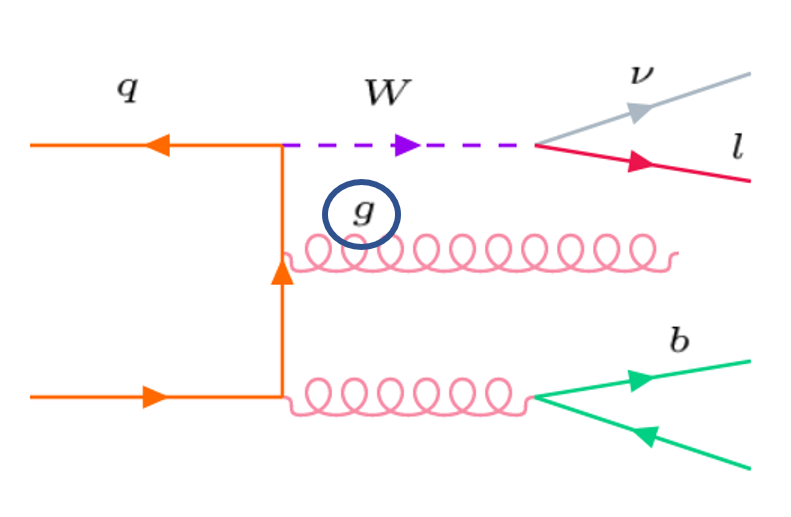
\includegraphics[width=.33\textwidth]{DiHiggs/plots/feynman_QCDfakes.png}
\caption{
Feynman diagrams on the left (right) for the \ttbar\ (multi-jet) with quark (gluon) circled in
red (blue) misidentified as a \tauhad. 
}
\label{fig:fakes:feynman}
\end{figure} 
Due to the different origins of the fake-\tauhad, the FF are
calculated separately for the \ttbar\ and multi-jet, and for 1 and 3-prong \tauhad\ candidates.
For each process the $FF$ are calculated in a dedicated background enriched region (FF-CR,
not to be confused with the CR used for statistical analysis). 
The FF-CRs for each process are defined as follows:
\begin{itemize}
\item \ttbar\ FF-CR: \mbb\ > 150 GeV, 2 $b$-tag 
\item Multi-jet (QCD) FF-CR: inverted lepton isolation 
	(`tight' electrons and `medium' muons are 
	required to fail their respective `loose' isolation working points), 
	2 $b$-tag. 
\end{itemize}
Individual fake factors for each process
are then used to provide a combined fake factor. 
The combined $FF$ is finally applied to the anti-\tauhad\ events 
to estimate the fake-\tauhad\ events in the SR.
The combined fake factor is defined as:
\begin{equation}
FF(\mathrm{comb}) = FF(\mathrm{QCD}) \times \mathrm{r}_{\mathrm{QCD}} + FF(\ttbar) \times (1 - \mathrm{r}_{\mathrm{QCD}}) 
\end{equation} 
where $\mathrm{r}_{\mathrm{QCD}}$ is measured as a function of the \tauhad\ \pT\ 
and defined as the fraction of multi-jet events in the anti-tau SR:
\begin{equation}
\mathrm{r}_{\mathrm{QCD}} = \frac{N(\mathrm{multi\mhyphen jet, data})} {N(\mathrm{data}) - N(\mathrm{true}~\tauhad, \mathrm{MC})}
\end{equation} 
and the $N(\mathrm{multi\mhyphen jet, data})$ is calculated by 
subtracting all background contributions apart from multi-jet, 
regardless of whether they contain fake or true-\tauhad\ candidates, 
from the data in the anti-\tauhad\ selection:
\begin{equation}
	N(\mathrm{multi\mhyphen jet, data}) = N(\mathrm{data}) - N(\mathrm{true}~\tauhad, \mathrm{MC} + \mathrm{fake}~\tauhad, \mathrm{MC})
\end{equation}  
The subtracted backgrounds are taken from the MC predictions. 
In graphical form, the various FF-CRs 
where the fake factors are measured and applied can be seen in Figure~\ref{fig:CombFFMethod}.
\begin{figure}[htbp]
\centering
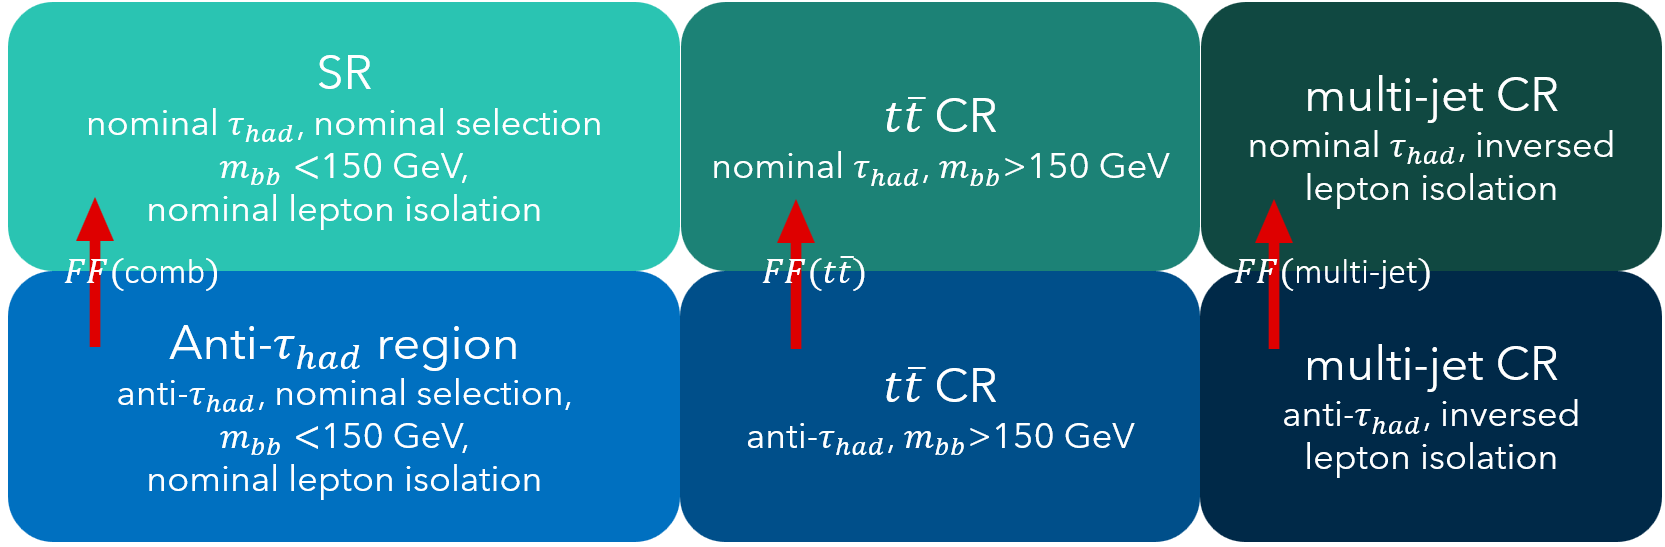
\includegraphics[width=.9\textwidth]{DiHiggs/plots/FF regions.png}
\caption{Graphical representation of the Combined Fake Factor Method. 
The fake factors are calculated independently for the \ttbar\ FF-CR and the multi-jet FF-CR, and 
combined to the combined fake factor. 
The direction of the arrow indicates the direction 
of extrapolation, 
that the FF is applied on the bottom regions to extrapolate to the top regions.}
\label{fig:CombFFMethod}
\end{figure}
The fake factor is parameterized in \pt\ of the \tauhad, where it shows an obvious trend.
The dependence on $\eta$ of the \tauhad\ is also checked but no clear trend is found.



The determination of the combined fake factor 
is sensitive to the modelling of simulated $t\bar{t}$ events with true-\tauhad\
given that this is the dominant background that is subtracted from data in the derivation of
the FFs and $\mathrm{r}_\text{QCD}$, and when obtaining the SR Template. Additionally, the derivation
of $\mathrm{r}_\text{QCD}$ is sensitive to the modelling of simulated $t\bar{t}$ events with fake-\tauhad.
It was observed that mismodeling in the \ttbar\ background 
especially in the high jet multiplicity and high top-quark \pt\ region
can cause issues in the calculation of the fake factors, 
giving non-physical negative values at high \tauhad\ \pt\ region. 
To mitigate this issue,
simulated events from $t\bar{t}$ production are differentially reweighted
depending on the jet multiplicity and the scalar sum of the transverse momentum of all visible
final state objects in the event.
These reweighting factors are determined from another $t\bar{t}$ FF-CR ($t\bar{t}$ FF-CR2),
% which is about 93\% pure in the events from $t\bar{t}$ production,
which is defined using a selection identical to the SR selection,
but with the \ttbar\ FF-CR $m_{bb}$ requirements ($m_{bb}>150$~GeV)
and an additional $m^{W}_\text{T}>40$~GeV requirement. 
Furthermore, events in this region are required
to have a reconstructed \tauhad\ candidate, but this candidate is not required
to pass the RNN \tauhad\ identification criteria defined in Section~\ref{sec:rec:tau}.
The $m^{W}_\text{T}$ requirement is introduced to remove any potential contamination from multi-jet events.
The reweighting method is validated in two additional validation regions.
The reweighting only applies to the FF-CRs and the anti-\tauhad\ regions, 
while it's not applying to the SR 
where the uncertainties due to the \ttbar\ modelling is accounted differently.   
% it would complicate the \ttbar\ systematics uncertainties and statistical analysis.
The \ttbar\ FF-CR and multi-jet FF-CR events with an anti-\tauhad\ candidate after the \ttbar\ reweighting 
are shown in Figure~\ref{fig:ttbarCR_1}, \ref{fig:ttbarCR_3}, \ref{fig:InvCR_1} and \ref{fig:InvCR_3}.
These plots can also be used to check the purity of the fake-\tauhad\ events in the \ttbar\ and multi-jet FF-CRs,  
where the fakes contributions from \ttbar\ are given from MC simulation.
In the multi-jet FF-CR, the events show large discrepancy between the
data and the MC distributions, as a result of the fakes originating from the 
multi-jet processes which are not simulated by the MC. 
A much larger fraction of \ttbar\ fakes are presented in the \ttbar\ FF-CR. 
The MC does not agree with data very well due to the imperfect \ttbar\ fakes MC simulation,
which is also the main motivation for using the data-driven FF method. 

\begin{figure}[htbp]
\centering
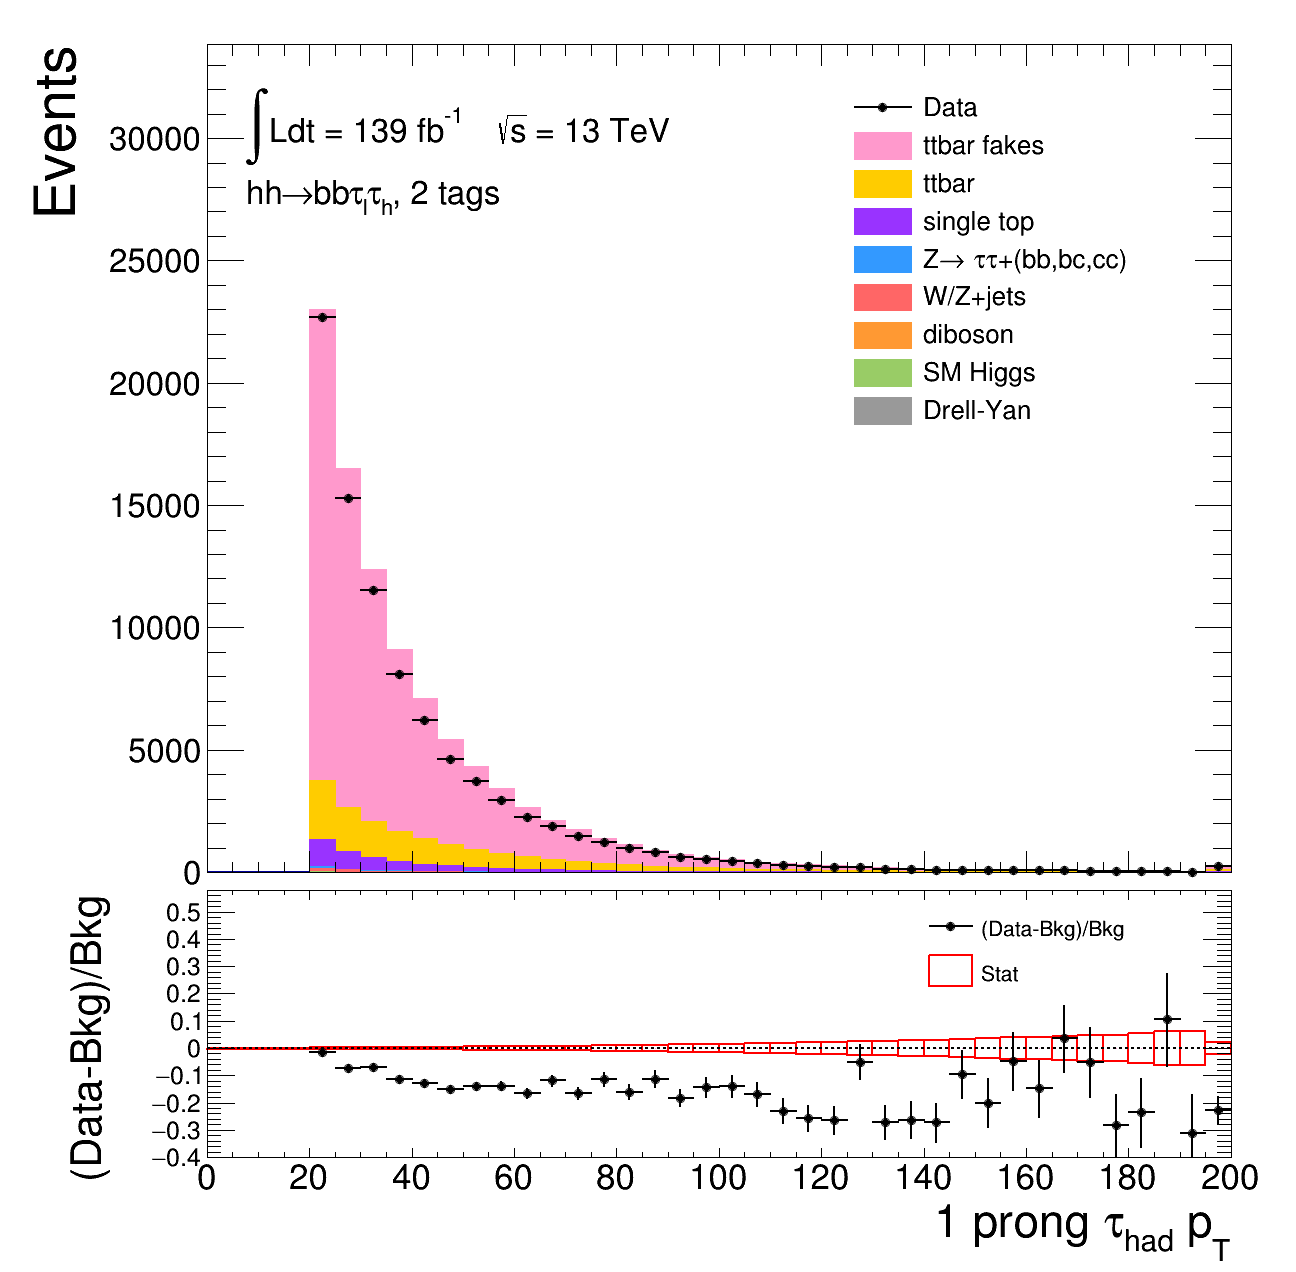
\includegraphics[width=.45\textwidth]{DiHiggs/plots/FF_CRs/ttbarCR_SLT/HNone/BDTVarsHighMbb/2/C_2tag2pjet_0ptv_TauPt1P.png}
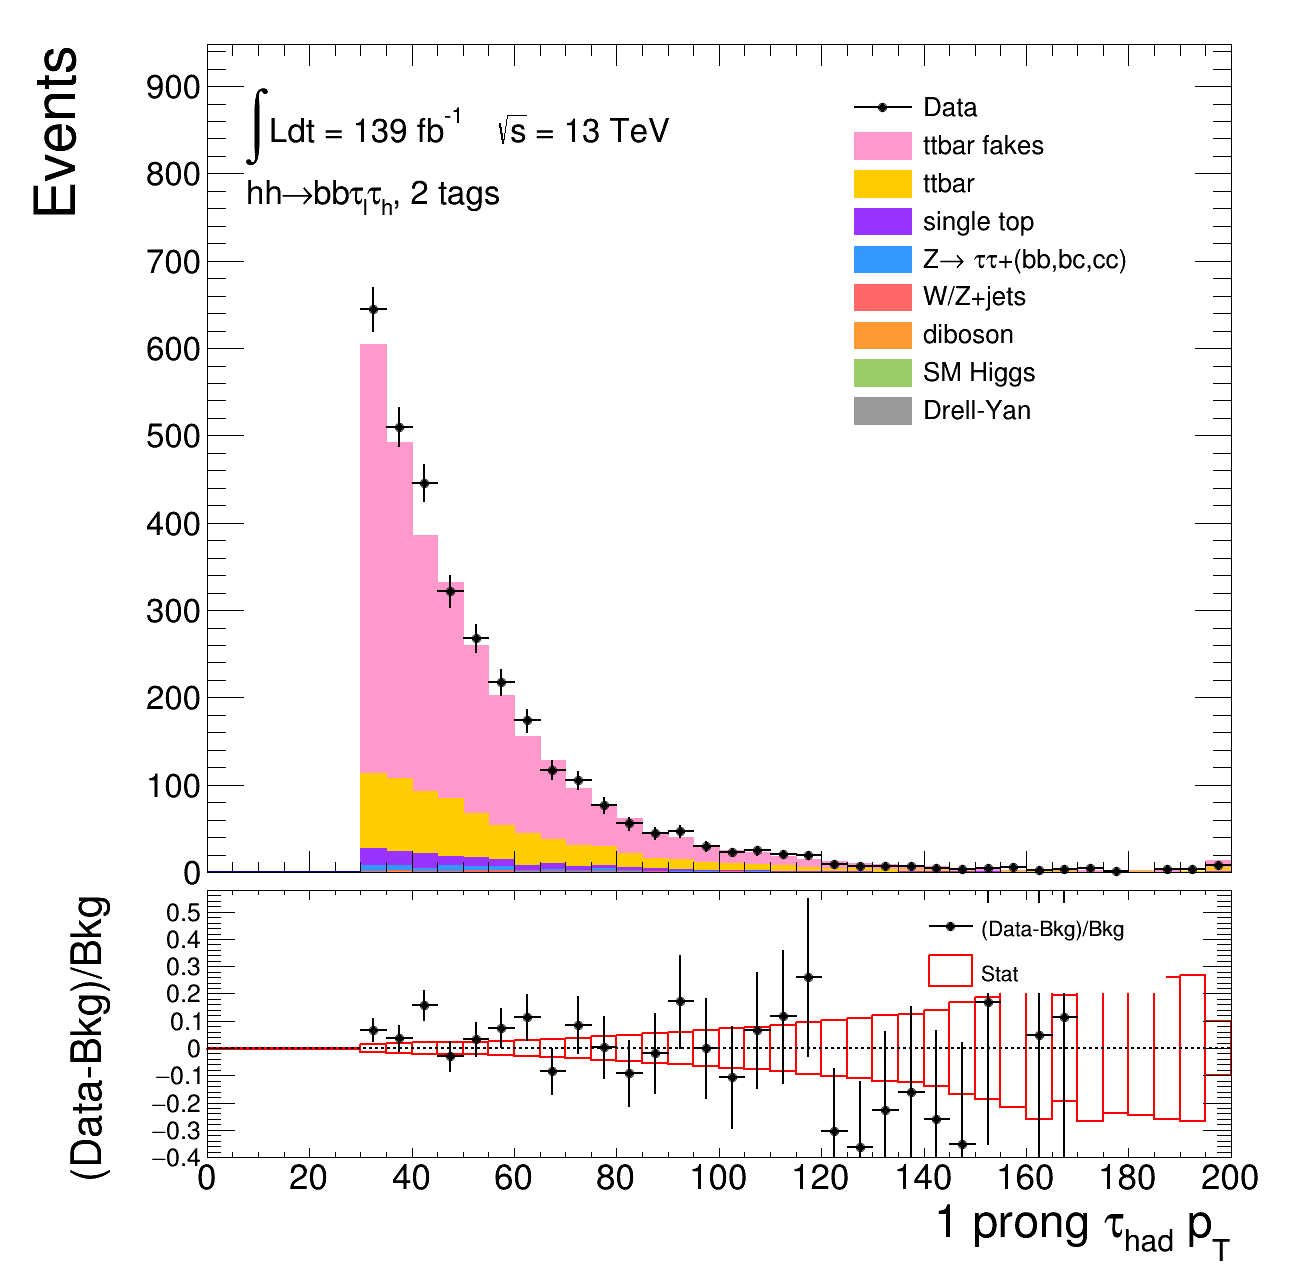
\includegraphics[width=.45\textwidth]{DiHiggs/plots/FF_CRs/ttbarCR_LTT/HNone/BDTVarsHighMbb/2/C_2tag2pjet_0ptv_TauPt1P.png}\\
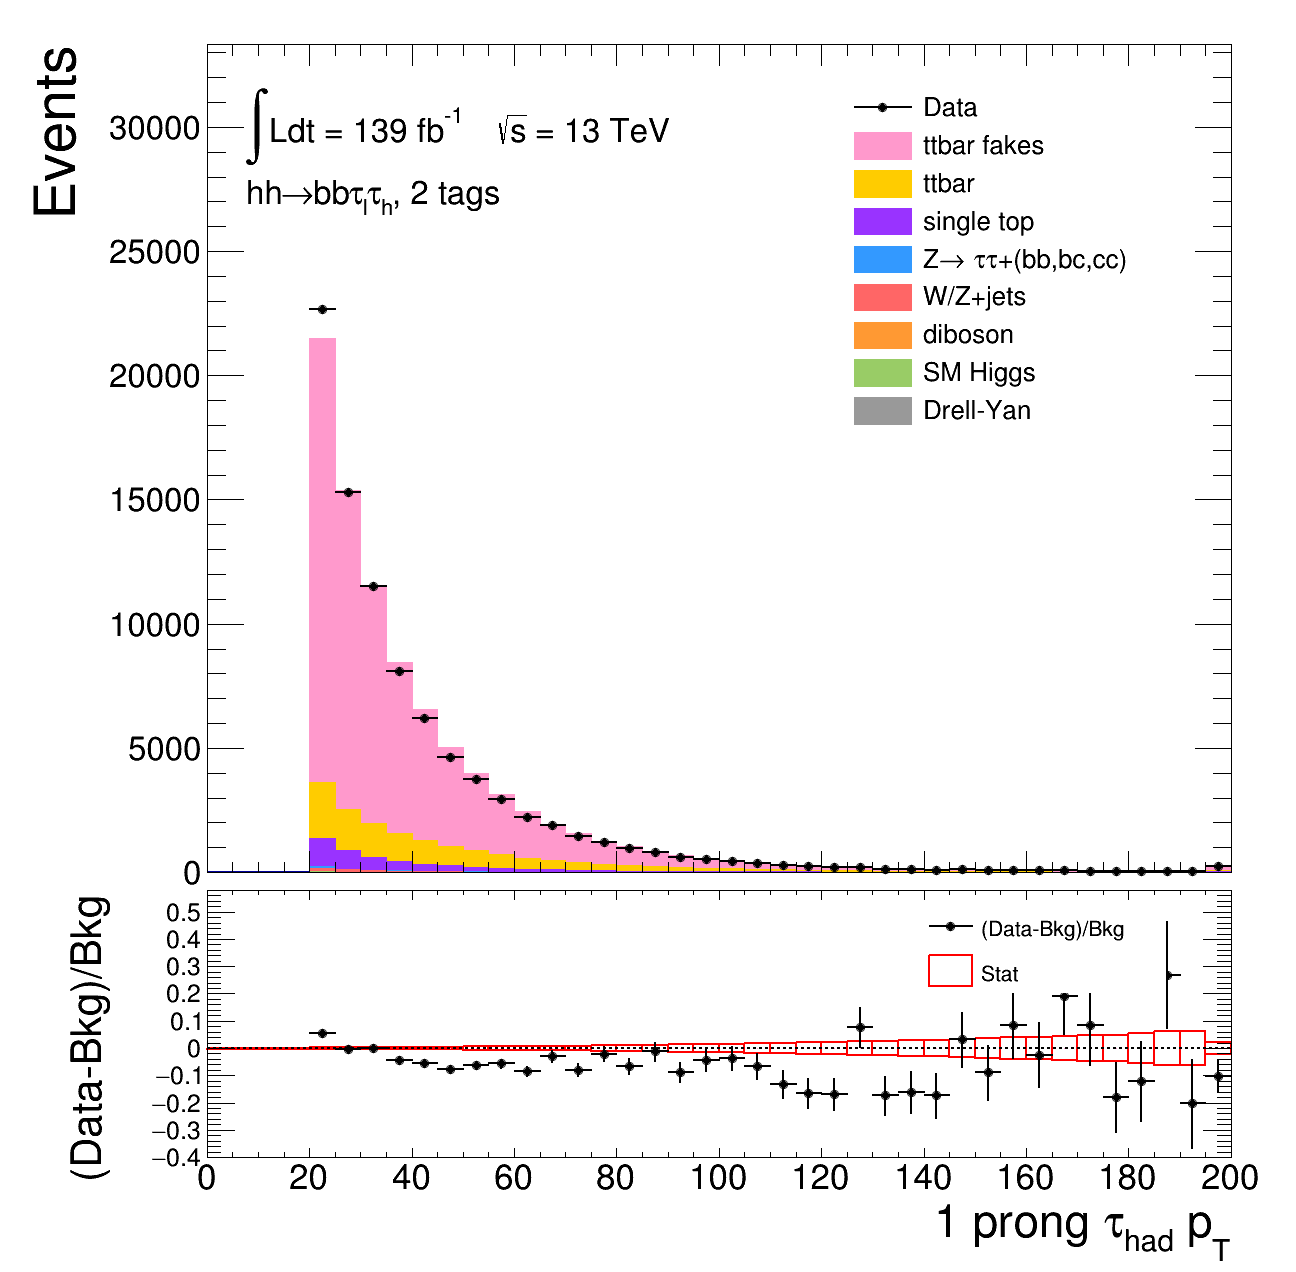
\includegraphics[width=.45\textwidth]{DiHiggs/plots/FF_CRs/ttbarCR_SLT_weighted/HNone/BDTVarsHighMbb/2/C_2tag2pjet_0ptv_TauPt1P.png}
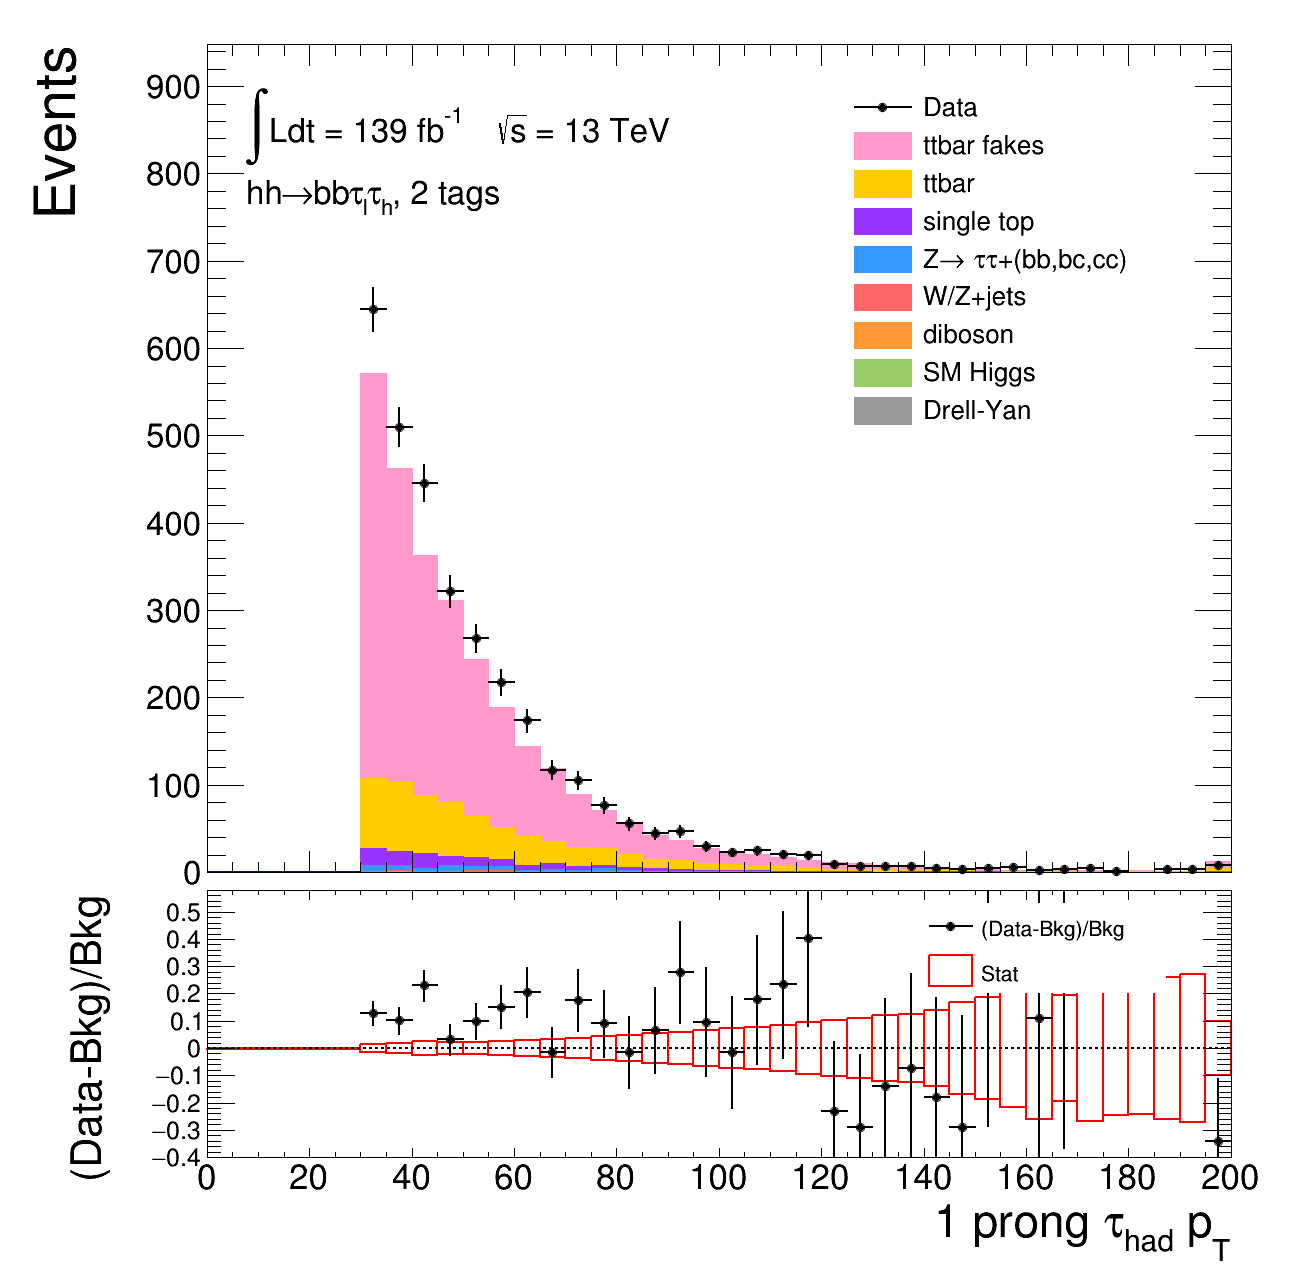
\includegraphics[width=.45\textwidth]{DiHiggs/plots/FF_CRs/ttbarCR_LTT_weighted/HNone/BDTVarsHighMbb/2/C_2tag2pjet_0ptv_TauPt1P.png}\\
\caption{Plots of the $\tauhad$ $p_T$ distributions for the SLT (left) and LTT channel (right) with \ttbar\ un-weighted (top)
and with \ttbar\ re-weighted (bottom) in the \ttbar\ FF-CR with 1-prong anti-\tauhad. 
The \ttbar\ initiated fakes background is labelled as `ttbar fakes' in pink.
With true \tauhad\ contributions subtracted from data (and with true \tauhad\ \ttbar\ reweighted),  
this region is used as the denominator of the \ttbar\ FF-CR fake factor calculation. 
Only statistical uncertainties are included.}
\label{fig:ttbarCR_1}
\end{figure} 
\begin{figure}[htbp]
\centering
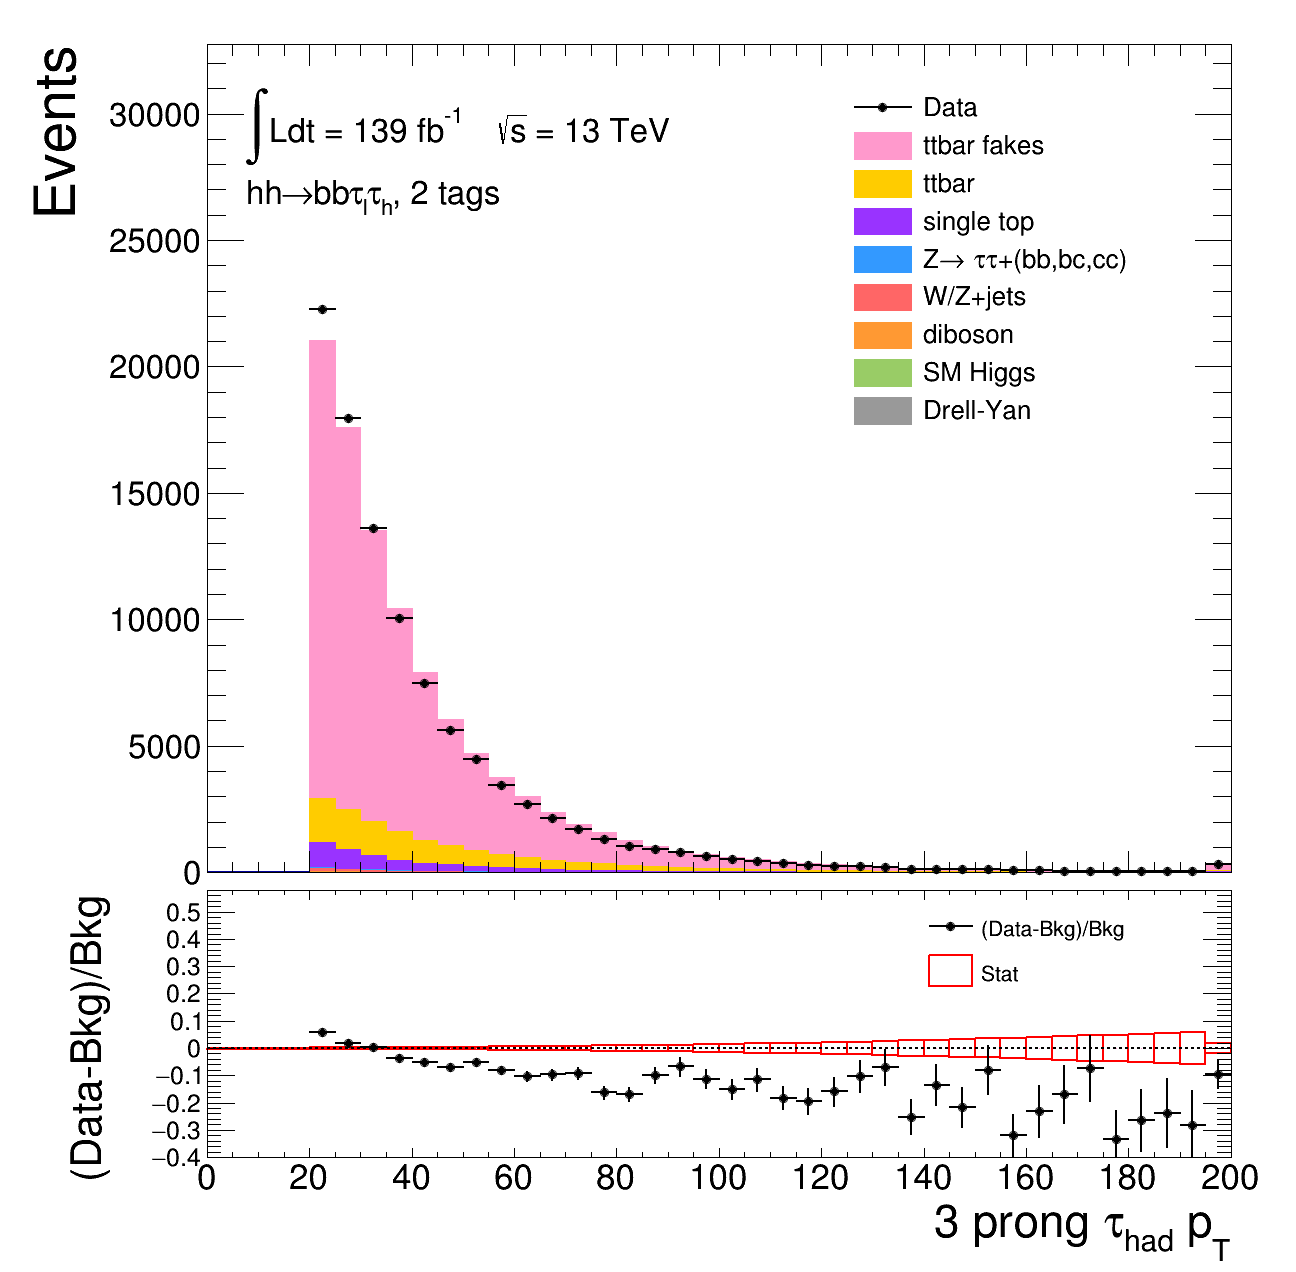
\includegraphics[width=.45\textwidth]{DiHiggs/plots/FF_CRs/ttbarCR_SLT/HNone/BDTVarsHighMbb/2/C_2tag2pjet_0ptv_TauPt3P.png}
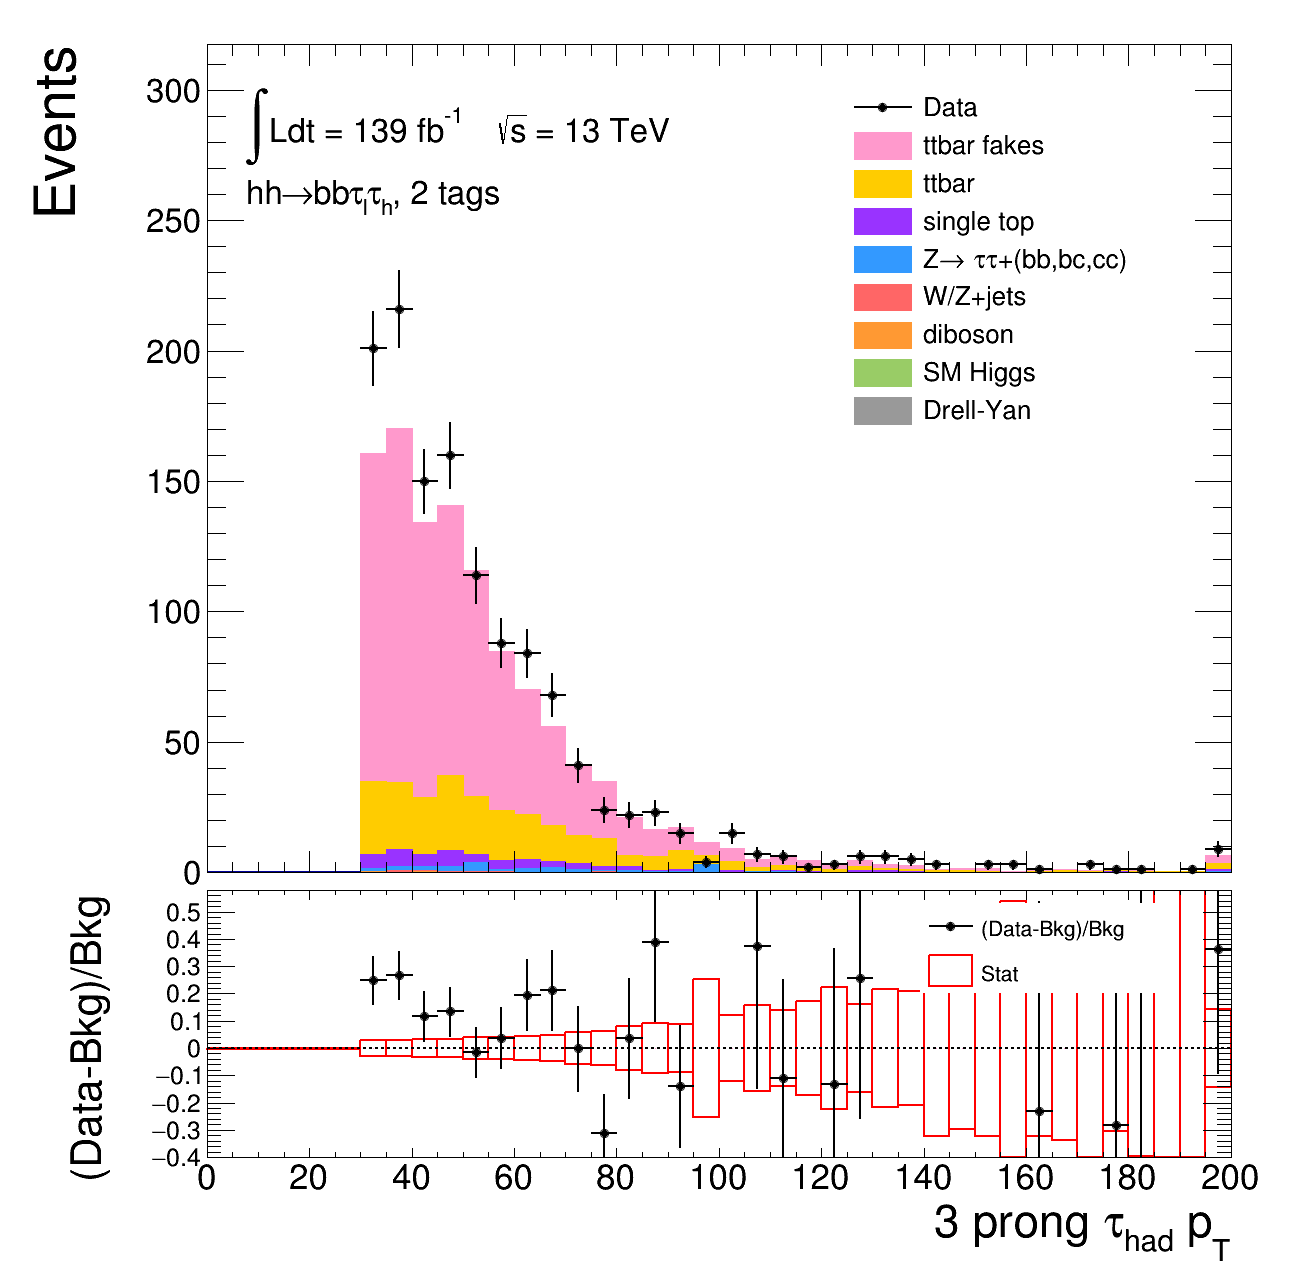
\includegraphics[width=.45\textwidth]{DiHiggs/plots/FF_CRs/ttbarCR_LTT/HNone/BDTVarsHighMbb/2/C_2tag2pjet_0ptv_TauPt3P.png}\\
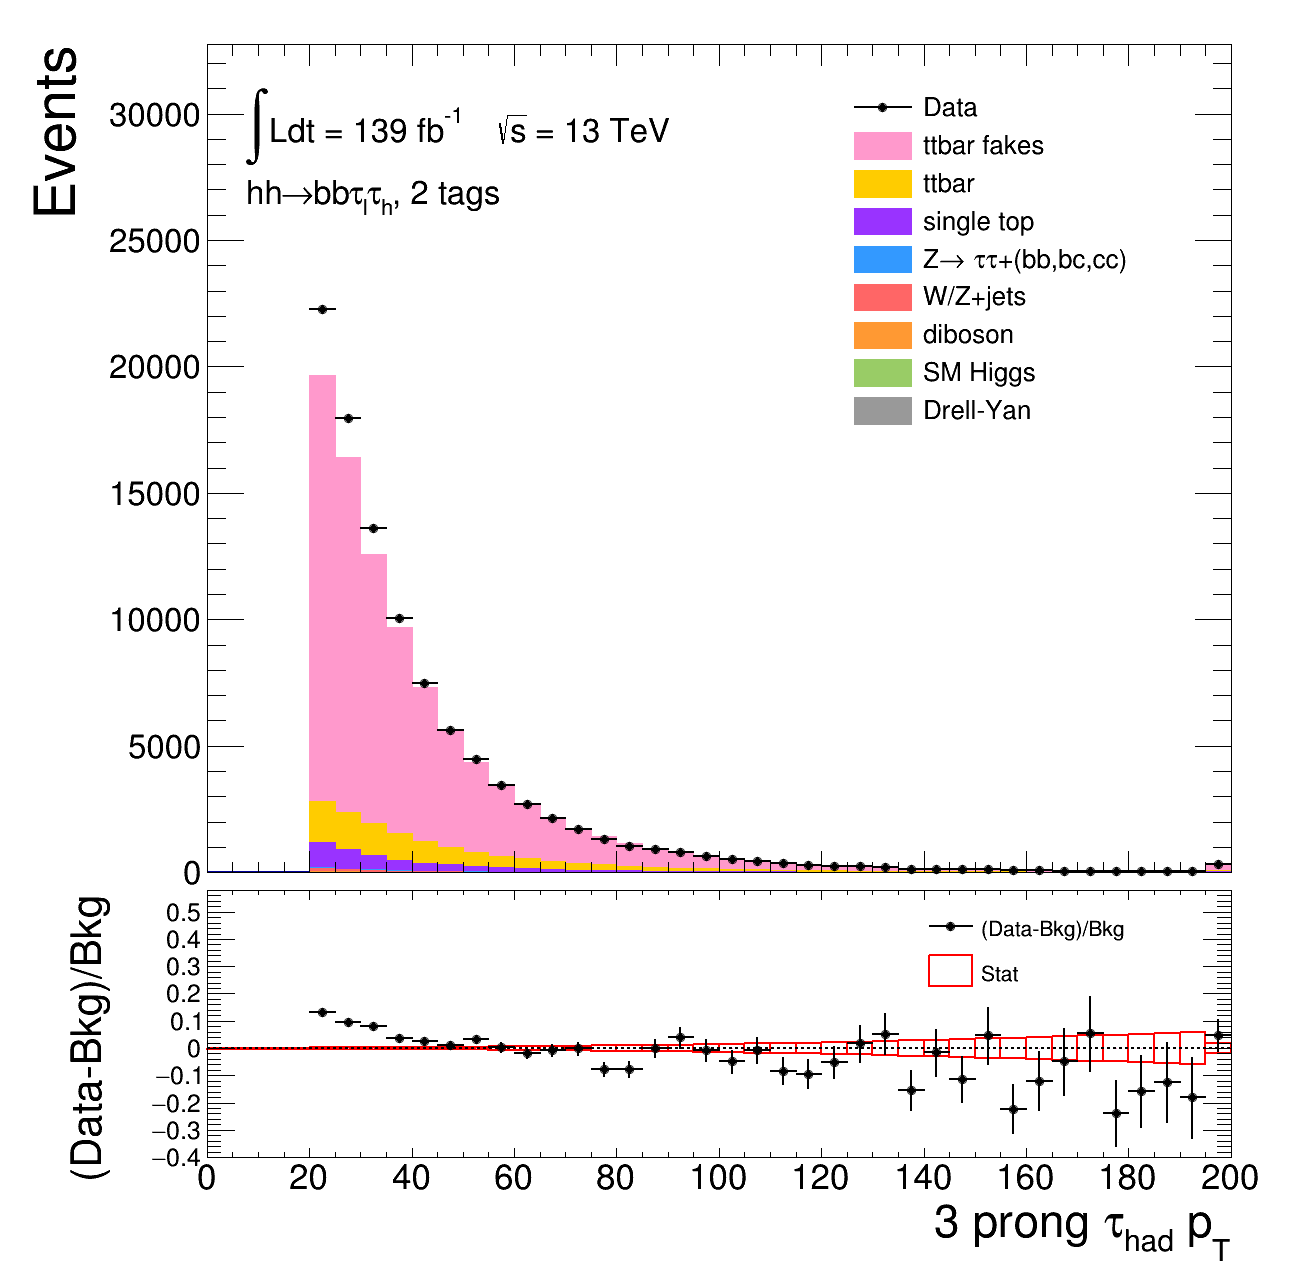
\includegraphics[width=.45\textwidth]{DiHiggs/plots/FF_CRs/ttbarCR_SLT_weighted/HNone/BDTVarsHighMbb/2/C_2tag2pjet_0ptv_TauPt3P.png}
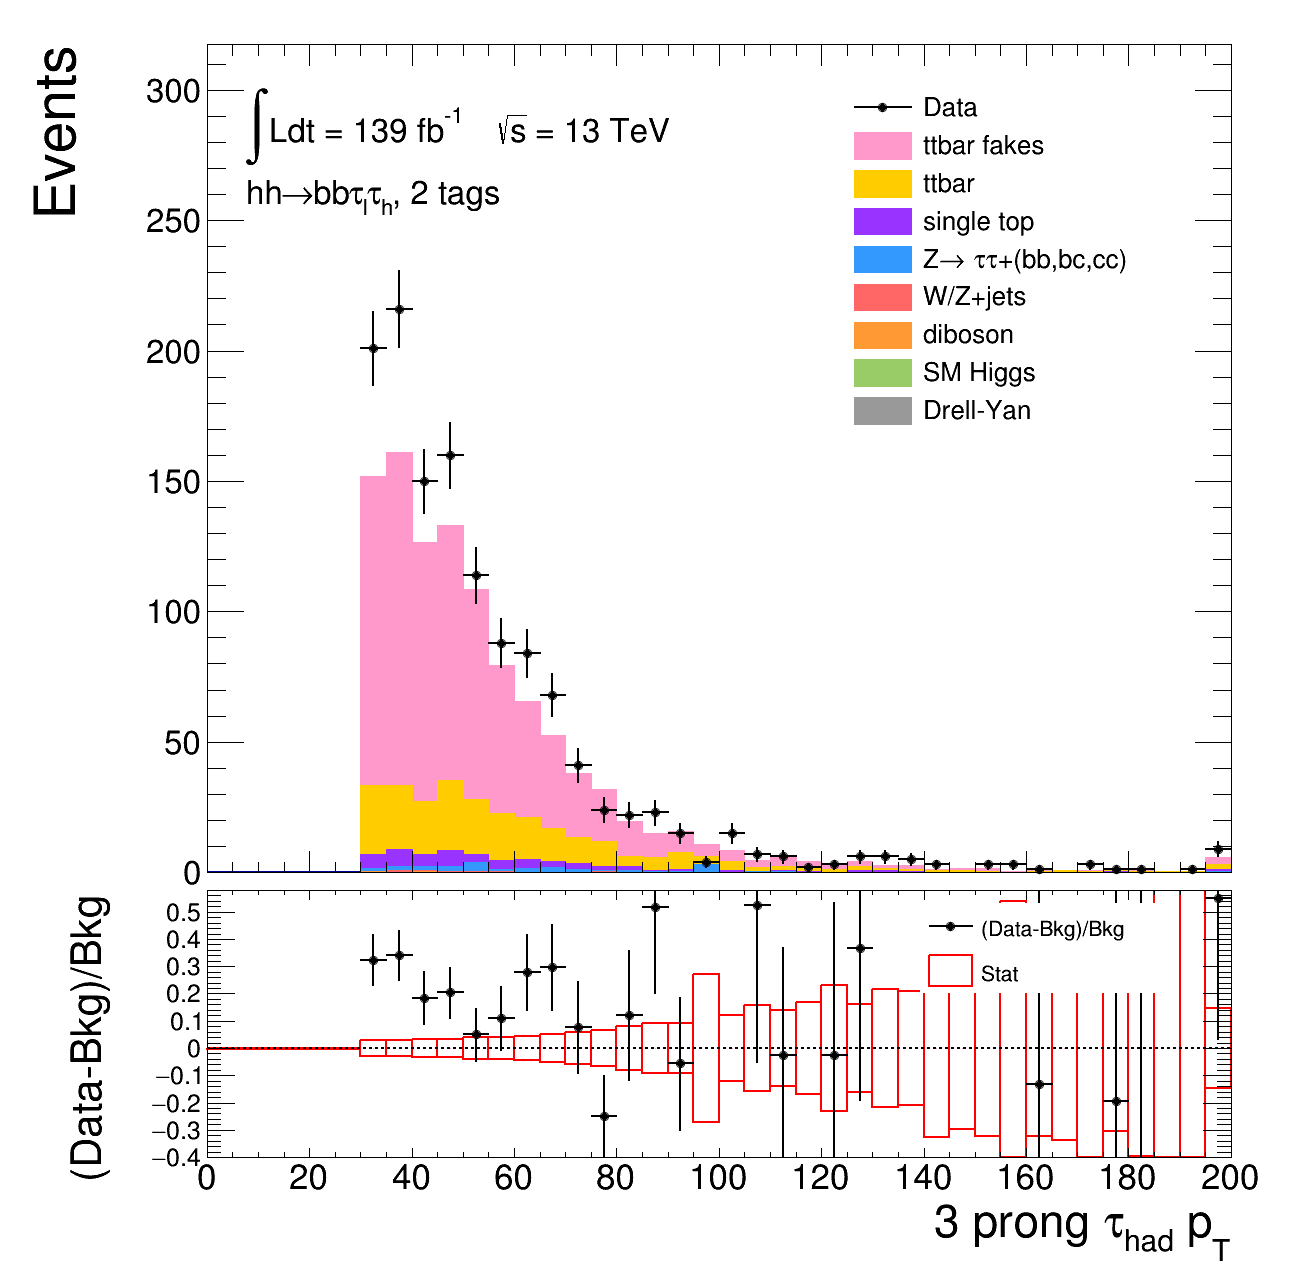
\includegraphics[width=.45\textwidth]{DiHiggs/plots/FF_CRs/ttbarCR_LTT_weighted/HNone/BDTVarsHighMbb/2/C_2tag2pjet_0ptv_TauPt3P.png}\\
\caption{Plots of the $\tauhad$ $p_T$ distributions for the SLT (left) and LTT channel (right) with \ttbar\ un-weighted (top)
and with \ttbar\ reweighted (bottom) in the \ttbar\ FF-CR with 3-prong anti-\tauhad.
The \ttbar\ initiated fakes background is labelled as `ttbar fakes' in pink.
With true \tauhad\ contributions subtracted from data (and with true \tauhad\ \ttbar\ reweighted), 
this region is used as the denominator of the \ttbar\ FF-CR fake factor calculation. 
Only statistical uncertainties are included.}
\label{fig:ttbarCR_3}
\end{figure} 
\begin{figure}[htbp]
\centering
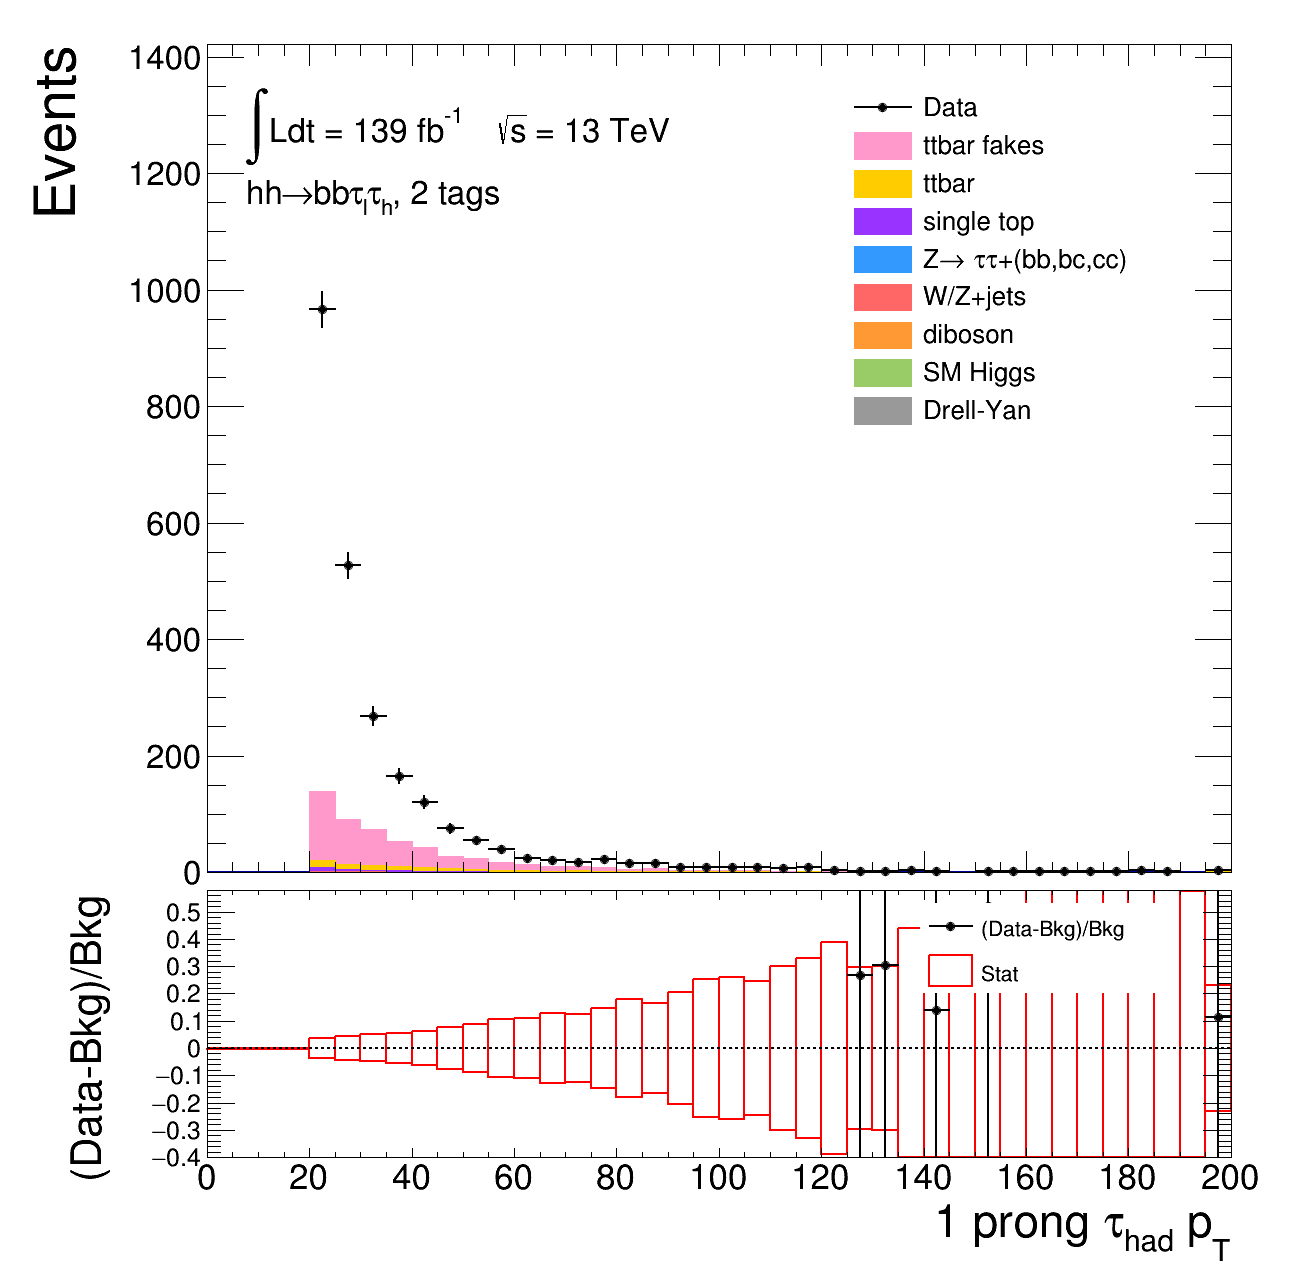
\includegraphics[width=.45\textwidth]{DiHiggs/plots/FF_CRs/InvCR_SLT/HNone/BDTVarsHighMbb/2/C_2tag2pjet_0ptv_TauPt1P.png}
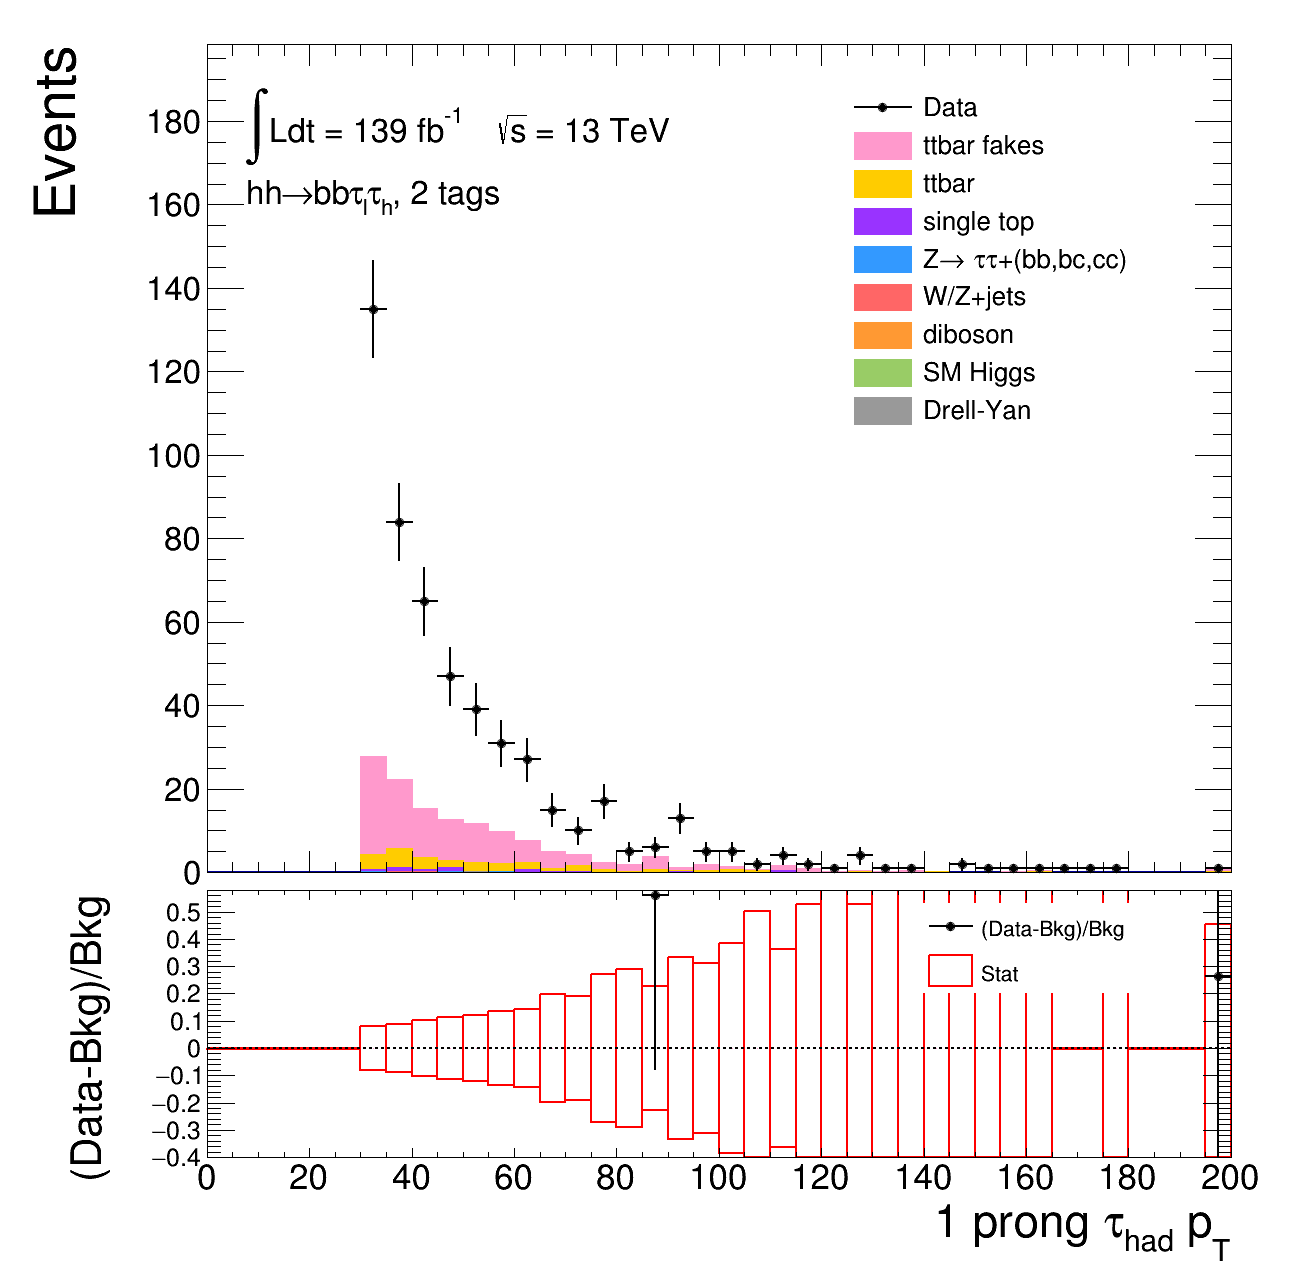
\includegraphics[width=.45\textwidth]{DiHiggs/plots/FF_CRs/InvCR_LTT/HNone/BDTVarsHighMbb/2/C_2tag2pjet_0ptv_TauPt1P.png}\\
\caption{Plots of the $\tauhad$ $p_T$ distributions for the SLT (left) and LTT channel (right) with \ttbar\ reweighted 
in the multi-jet FF-CR with 1-prong anti-\tauhad. 
The \ttbar\ initiated fakes background is labelled as `ttbar fakes' in pink.
With true \tauhad\ contributions subtracted from data, 
this region is used as the denominator of the \ttbar\ FF-CR fake factor calculation. 
Only statistical uncertainties are included.}
\label{fig:InvCR_1}
\end{figure} 

\begin{figure}[htbp]
\centering
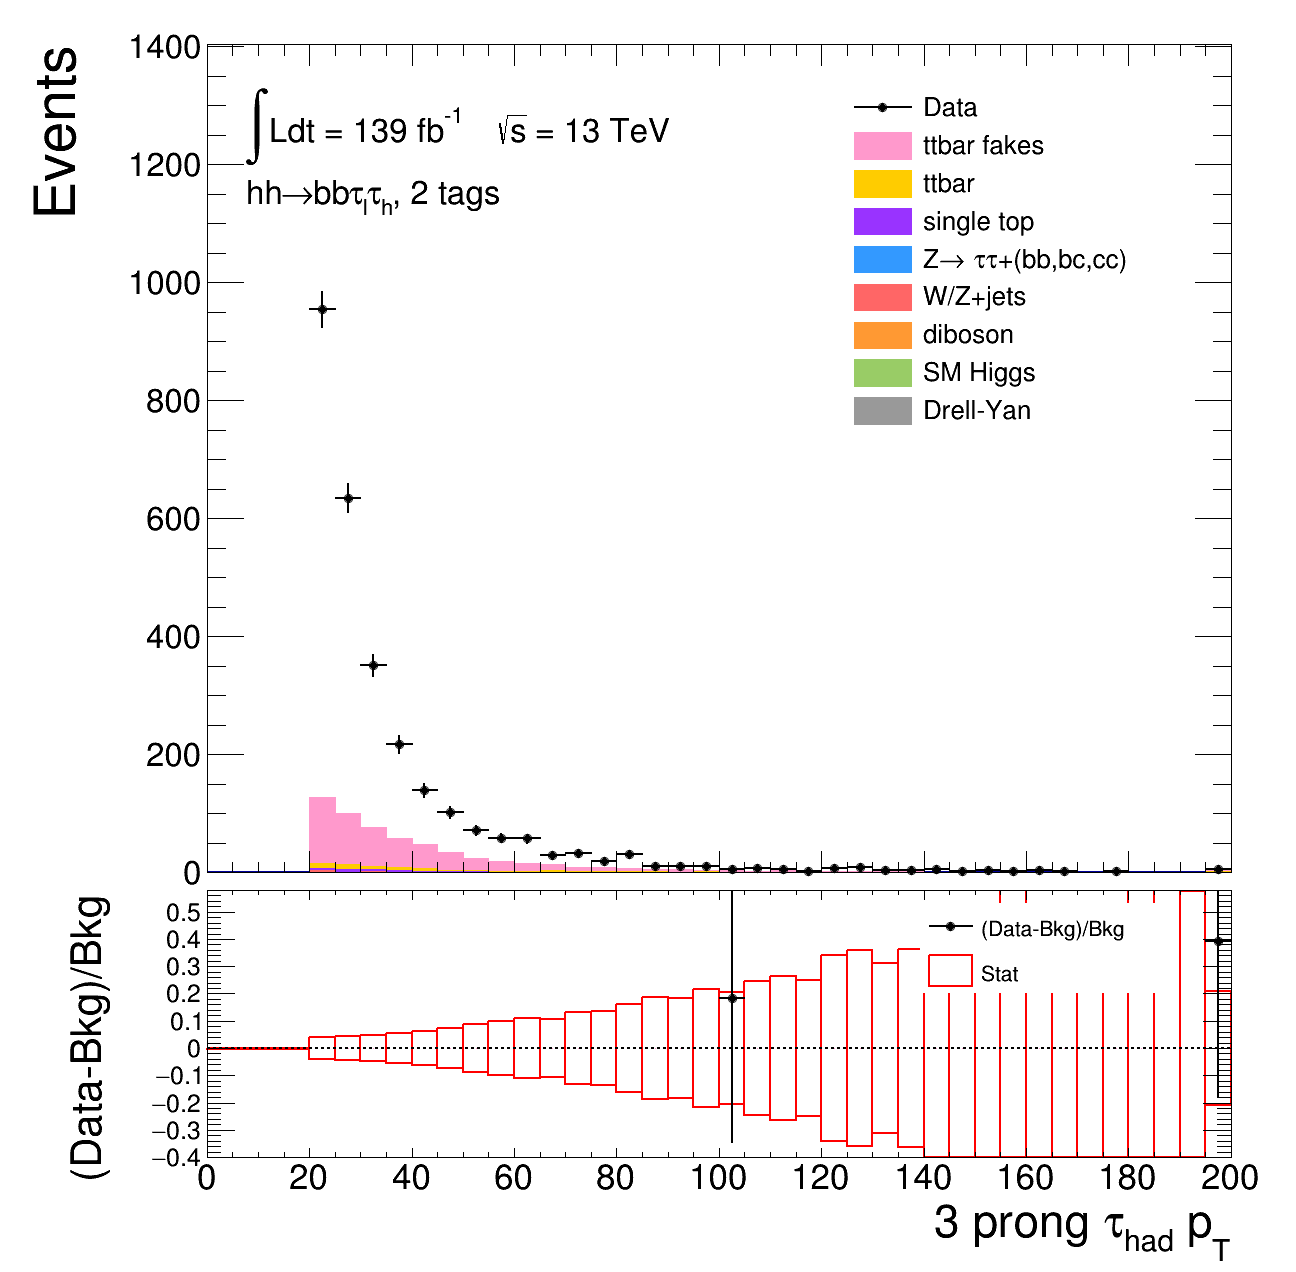
\includegraphics[width=.45\textwidth]{DiHiggs/plots/FF_CRs/InvCR_SLT/HNone/BDTVarsHighMbb/2/C_2tag2pjet_0ptv_TauPt3P.png}
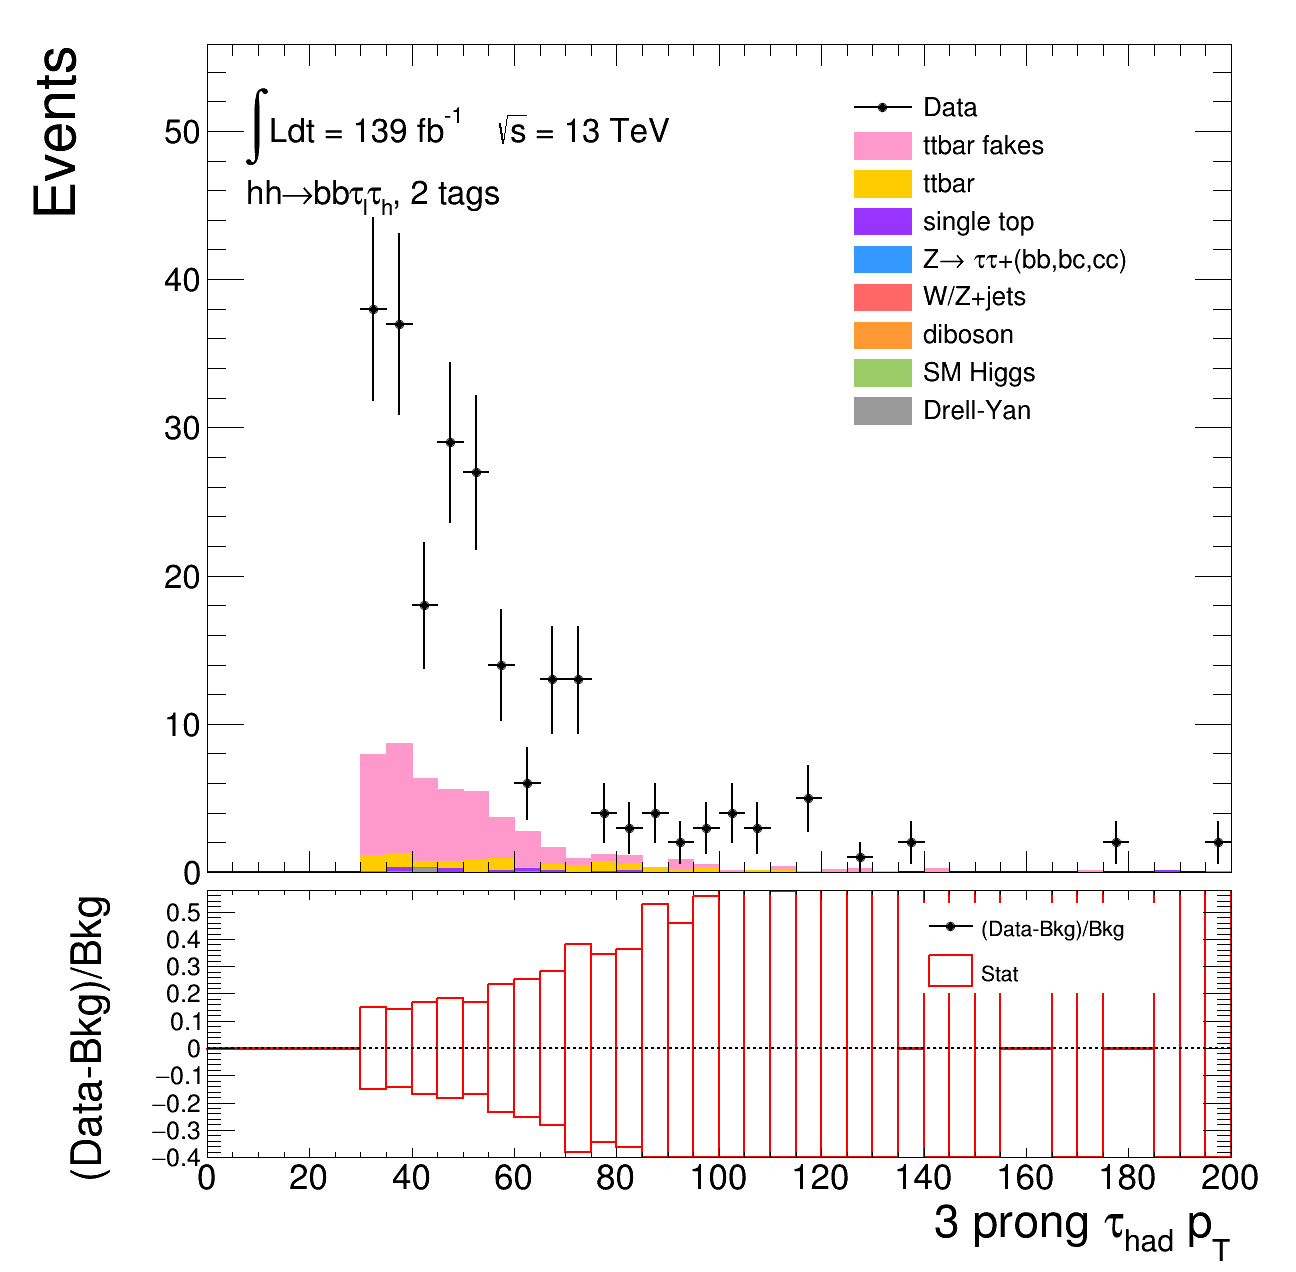
\includegraphics[width=.45\textwidth]{DiHiggs/plots/FF_CRs/InvCR_LTT/HNone/BDTVarsHighMbb/2/C_2tag2pjet_0ptv_TauPt3P.png}\\
\caption{Plots of the $\tauhad$ $p_T$ distributions for the SLT (left) and LTT channel (right) with \ttbar\ reweighted.
The \ttbar\ initiated fakes background is labelled as `ttbar fakes' in pink.
With true \tauhad\ contributions subtracted from data, 
this region is used as the denominator of the multi-jet FF-CR fake factor calculation. 
Only statistical uncertainties are included.}
\label{fig:InvCR_3}
\end{figure} 

The calculated fake factors are shown on Figure~\ref{fig:SLT_FF} and Figure~\ref{fig:LTT_FF}, 
for the SLT and LTT channels respectively. 
The Fake factors obtained with reweighted and un-weighted \ttbar\ contributions are shown on the
same graph. 
The binning is optimised for the $\text{FF}_{t\bar{t}}$ and the same binning is used for the 
$\text{FF}_\text{QCD}$. A smooth trend is observed in the $\text{FF}_{t\bar{t}}$, 
but some artifacts shapes at mid and high \pt\ range are showin in the $\text{FF}_\text{QCD}$.
This issue has no visible impact on the fakes estimation, because the 
the \ttbar\ FF dominates over the multi-jet FF in the combined FF which can be seen 
in the $\mathrm{r}_\text{QCD}$ distribution in Figure.~\ref{fig:SLT_rQCD} and Figure.~\ref{fig:LTT_rQCD}. 
The $\mathrm{r}_{\mathrm{QCD}}$ is computed both for $e\tauhad$ and $\mu\tauhad$ channels, 
since the QCD contents are different for them.
The parameterized $\mathrm{r}_{\mathrm{QCD}}$ 
as a function of \pT(\tauhad) for 1-prong and 3-prong \tauhad\ candidates in $e\tauhad$ and $\mu\tauhad$ channels 
are shown in Figure~\ref{fig:SLT_rQCD} for the SLT category and 
in Figure~\ref{fig:LTT_rQCD} for the LTT category.

Statistical uncertainties in $\text{FF}_{t\bar{t}}$, $\text{FF}_\text{QCD}$ and $\mathrm{r}_\text{QCD}$
are evaluated and propagated to the final result,
and a conservative 30\% modelling uncertainty is assigned to simulated non-$t\bar t$ backgrounds
which are subtracted from data.
The uncertainties due to \ttbar\ modelling issue and its subtraction are discussed in more details
in section~\ref{sec:DiHiggs:fakesysts}.TODO: add reference to the systematics section.

\begin{figure}[htbp]
\centering
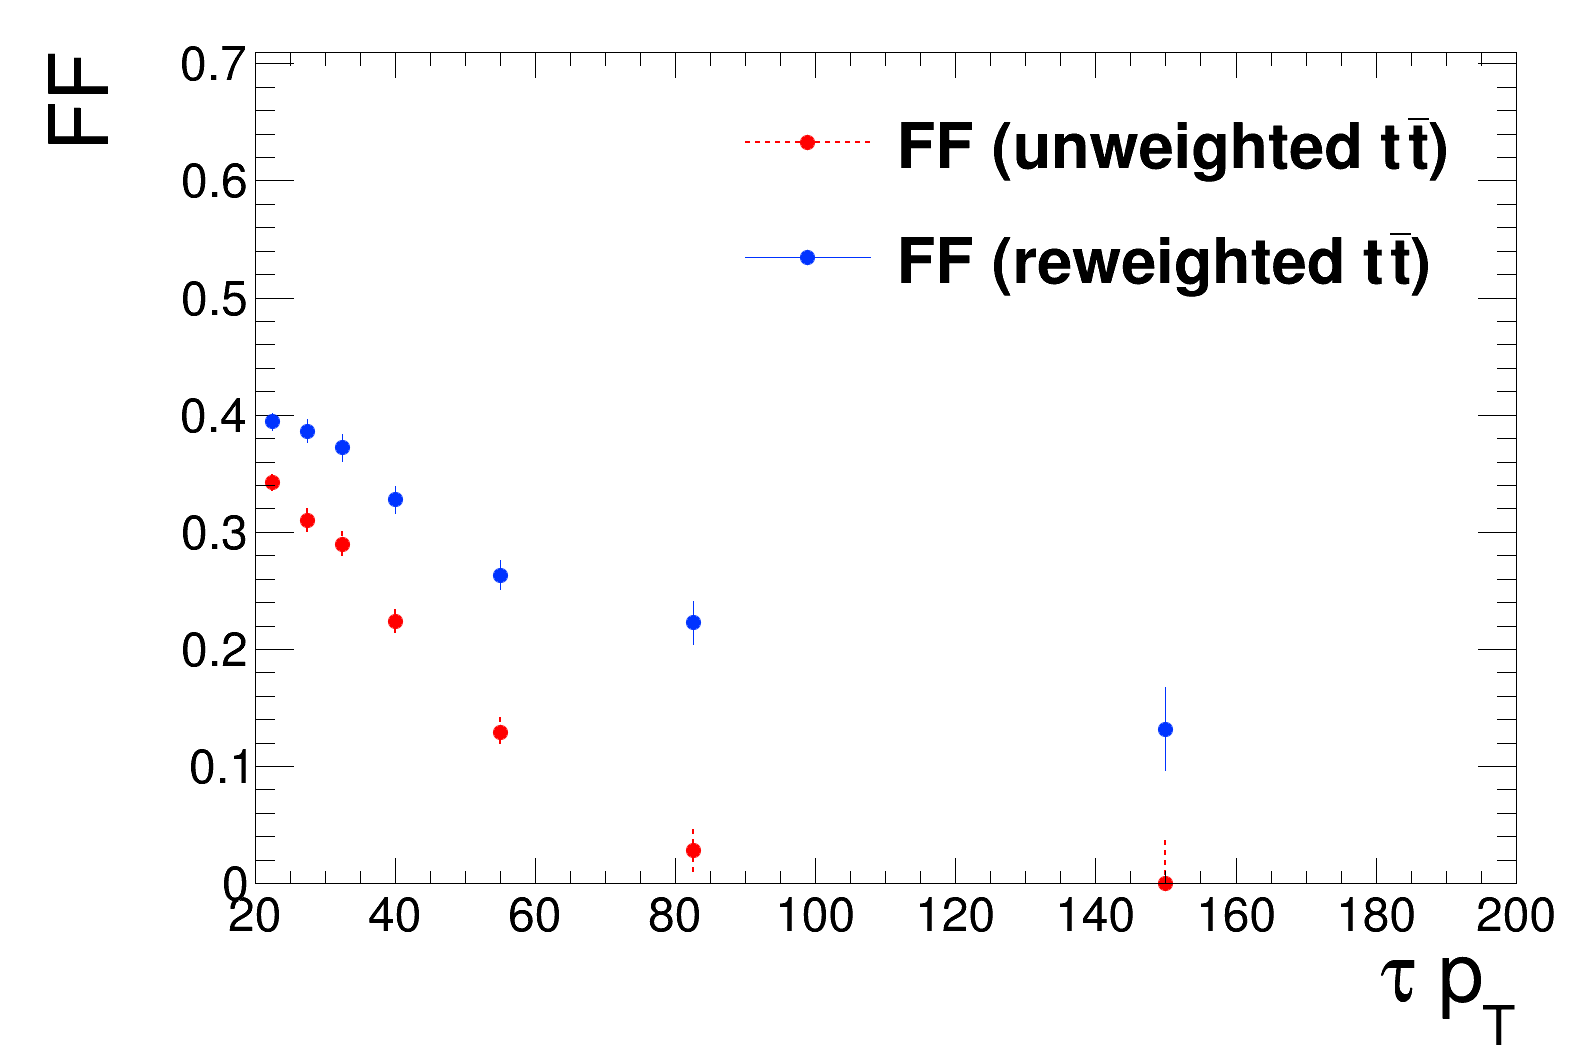
\includegraphics[width=.4\textwidth]{DiHiggs/plots/FF_CRs/SLTttbarCR1p.png}
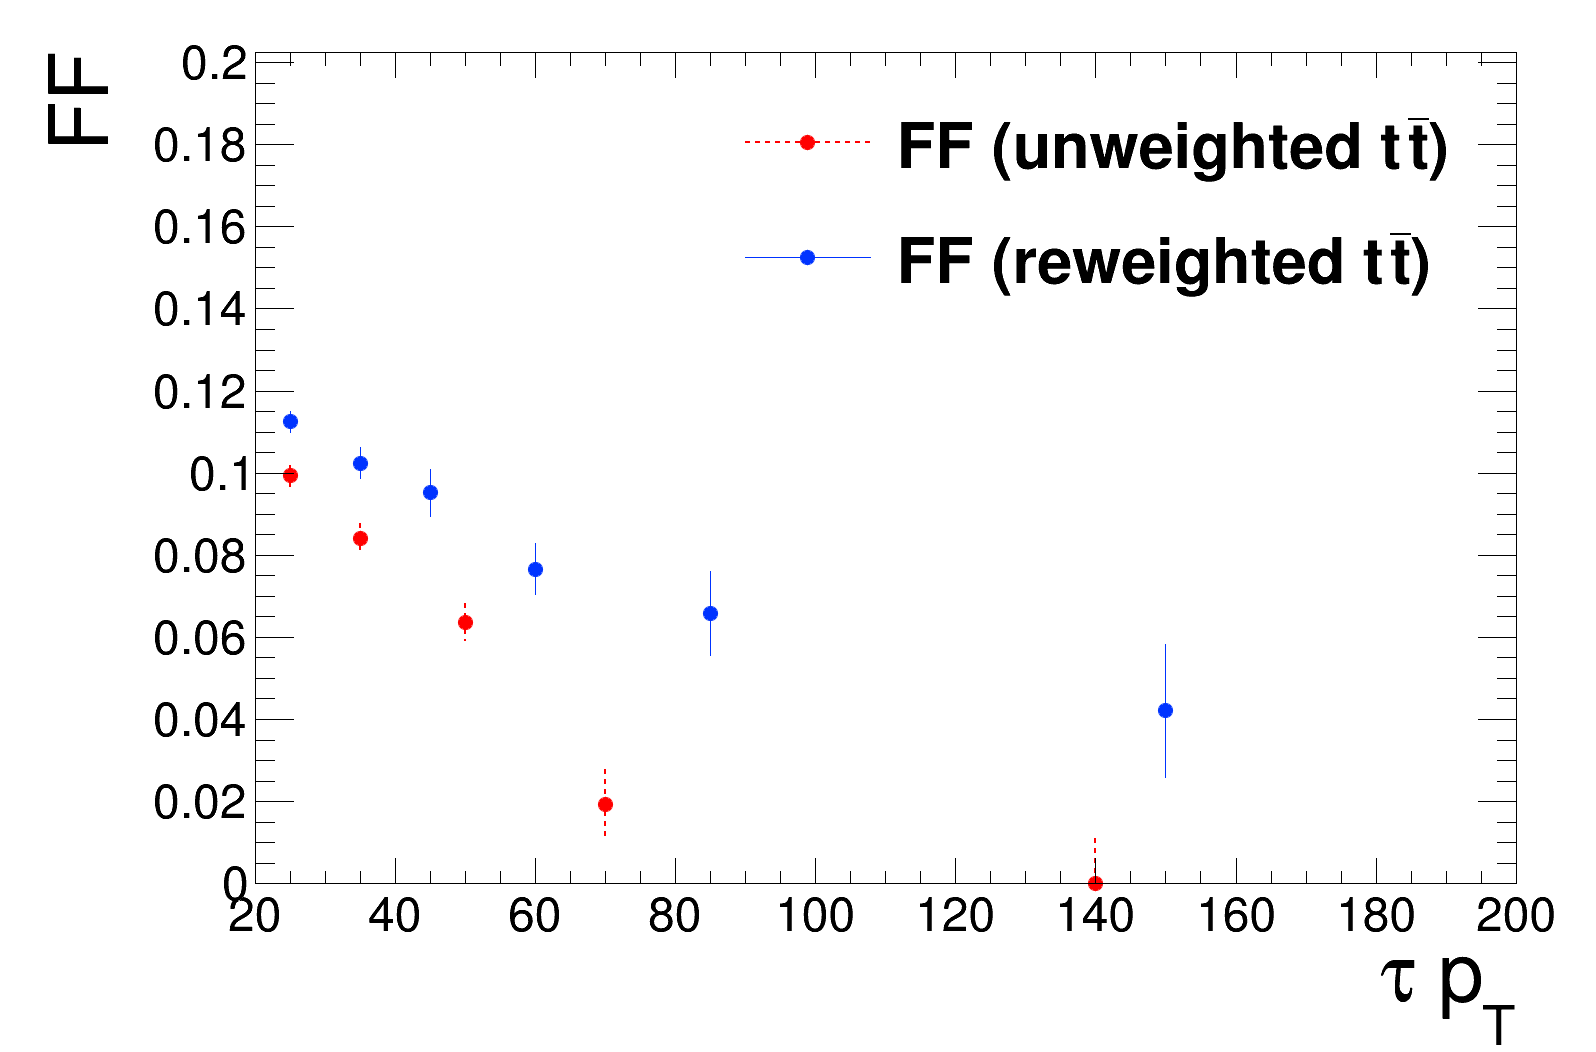
\includegraphics[width=.4\textwidth]{DiHiggs/plots/FF_CRs/SLTttbarCR3p.png} \\
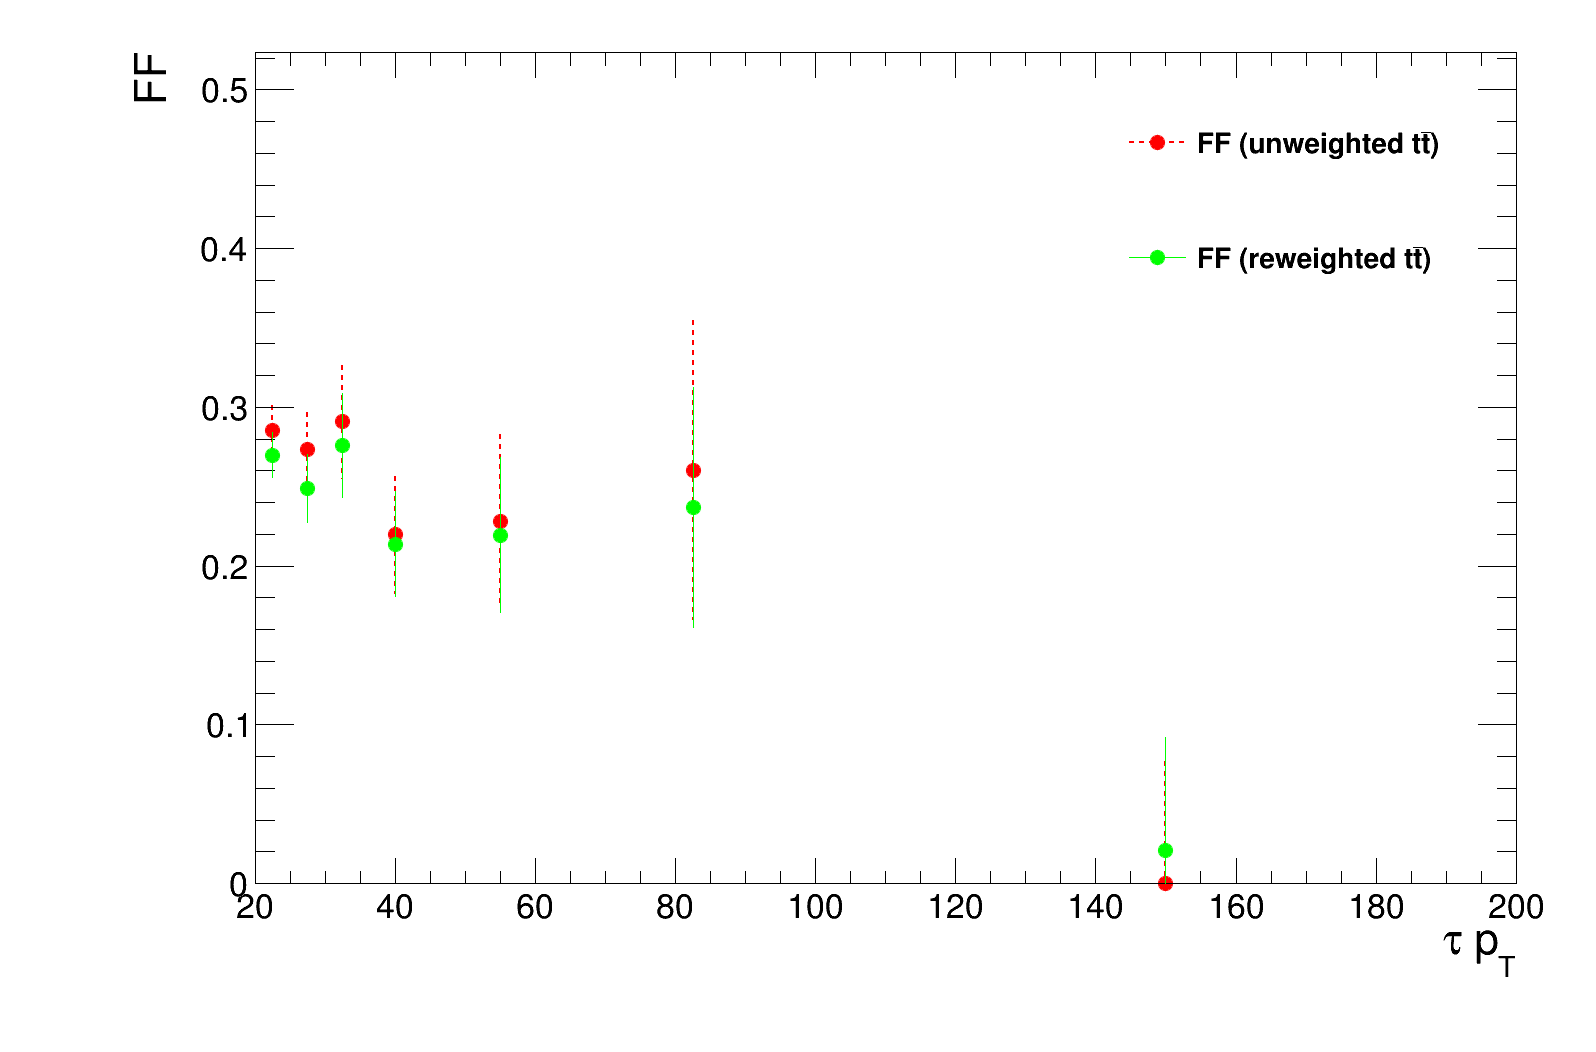
\includegraphics[width=.4\textwidth]{DiHiggs/plots/FF_CRs/SLTInvCR1p.png}
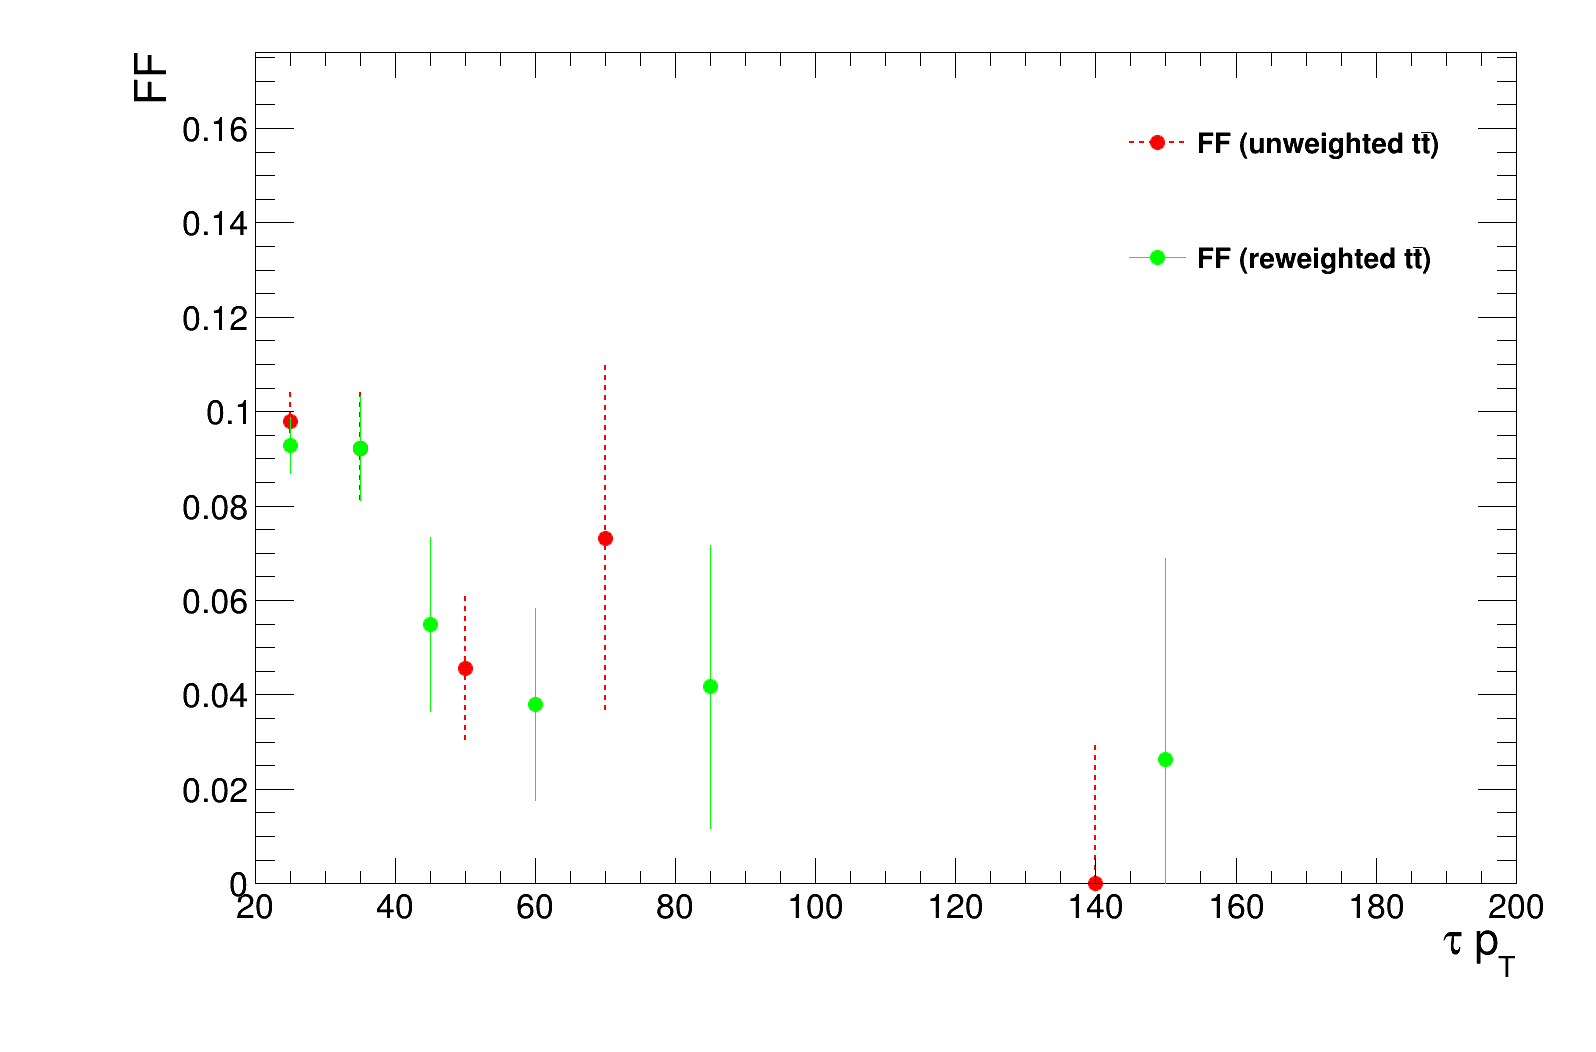
\includegraphics[width=.4\textwidth]{DiHiggs/plots/FF_CRs/SLTInvCR3p.png}\\
\caption{Fake factors for 1-prong (left) and 3-prong (right) \tauhad\ candidates for \ttbar\ processes (top) and multi-jet (bottom) for the \lephad SLT category.}
\label{fig:SLT_FF}
\end{figure}

\begin{figure}[htbp]
\centering
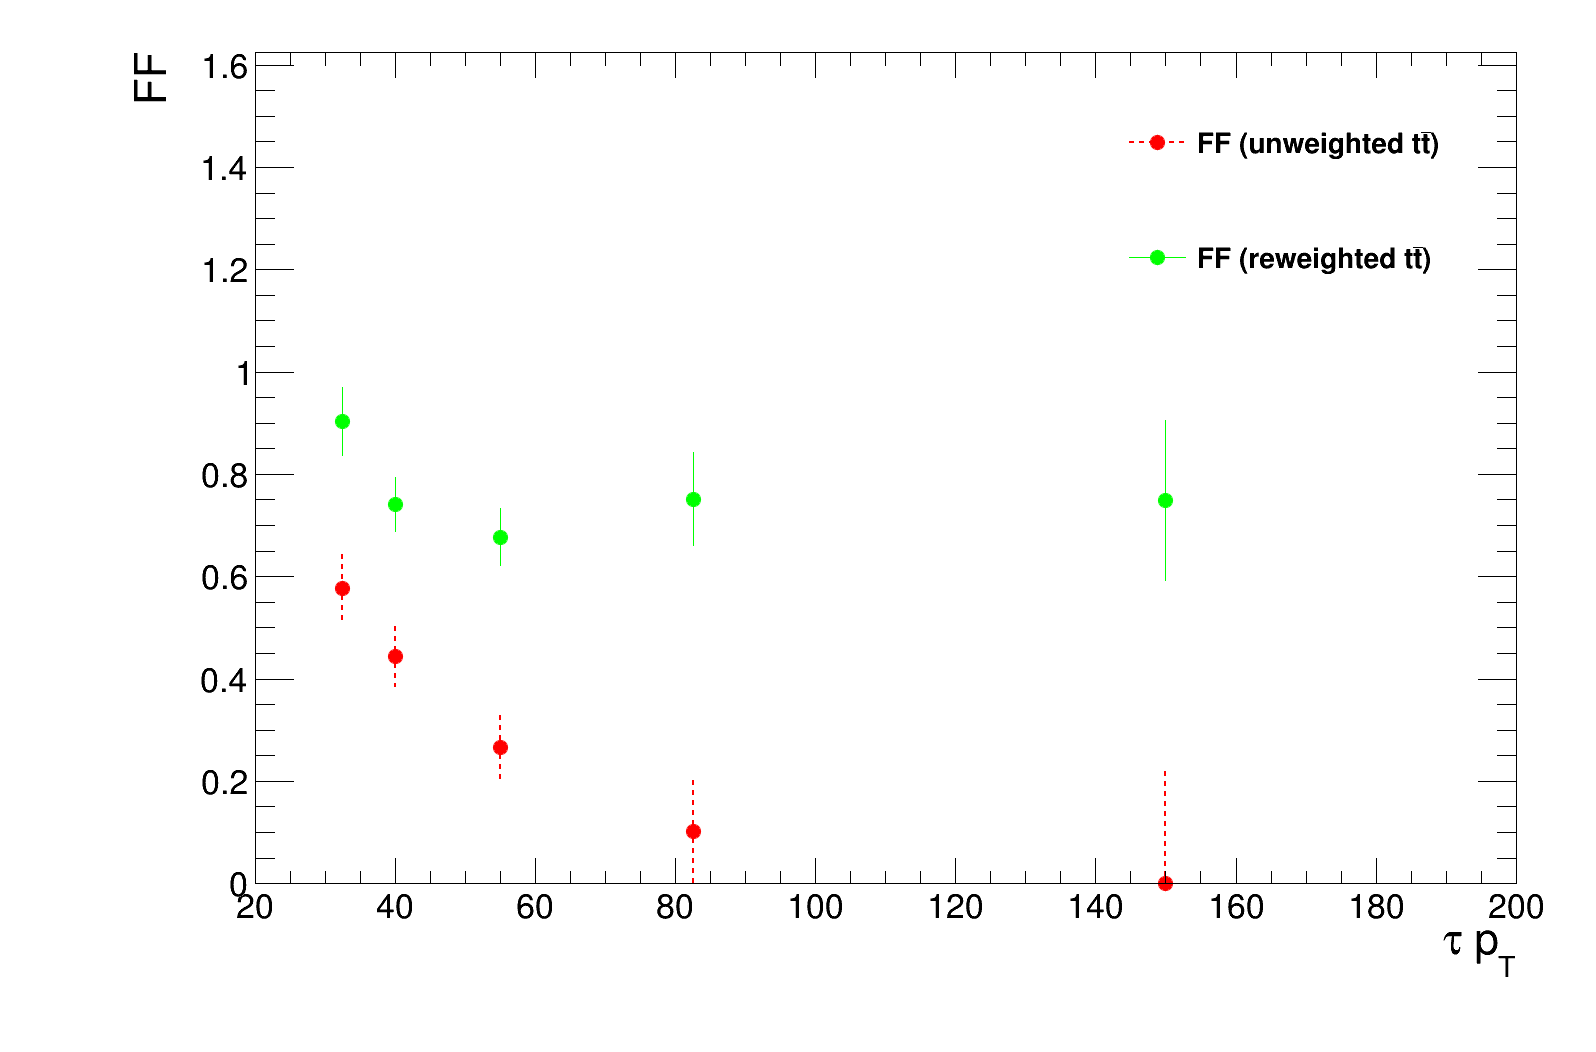
\includegraphics[width=.4\textwidth]{DiHiggs/plots/FF_CRs/LTTttbarCR1p.png}
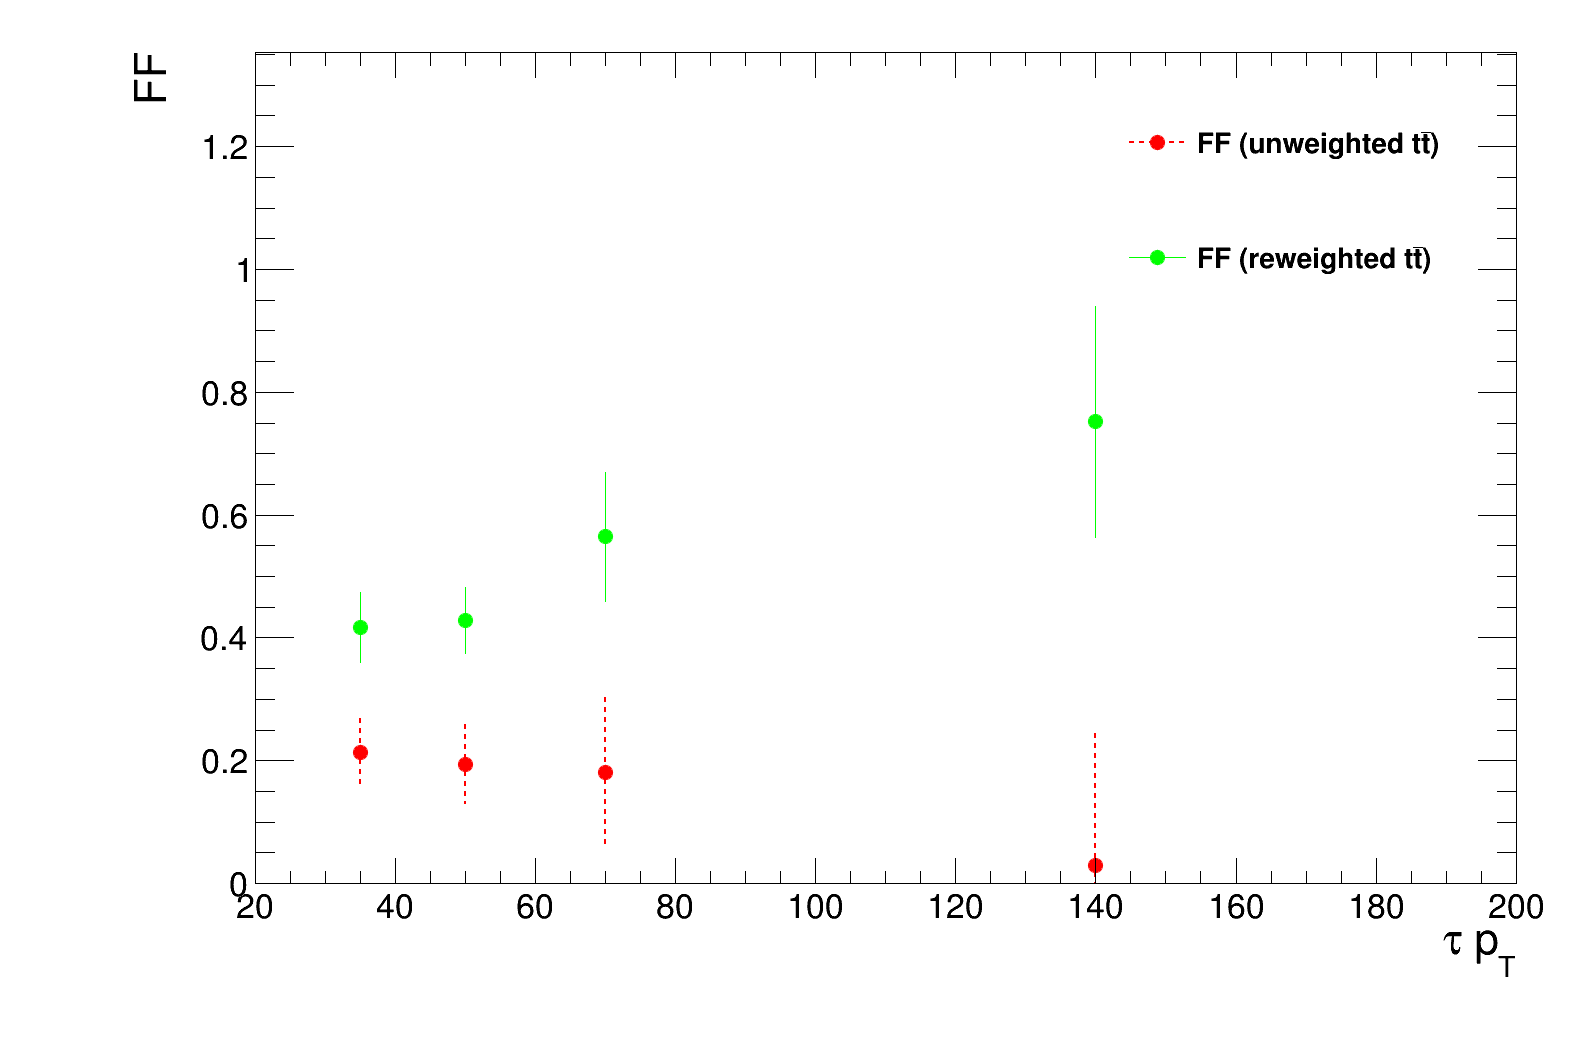
\includegraphics[width=.4\textwidth]{DiHiggs/plots/FF_CRs/LTTttbarCR3p.png} \\
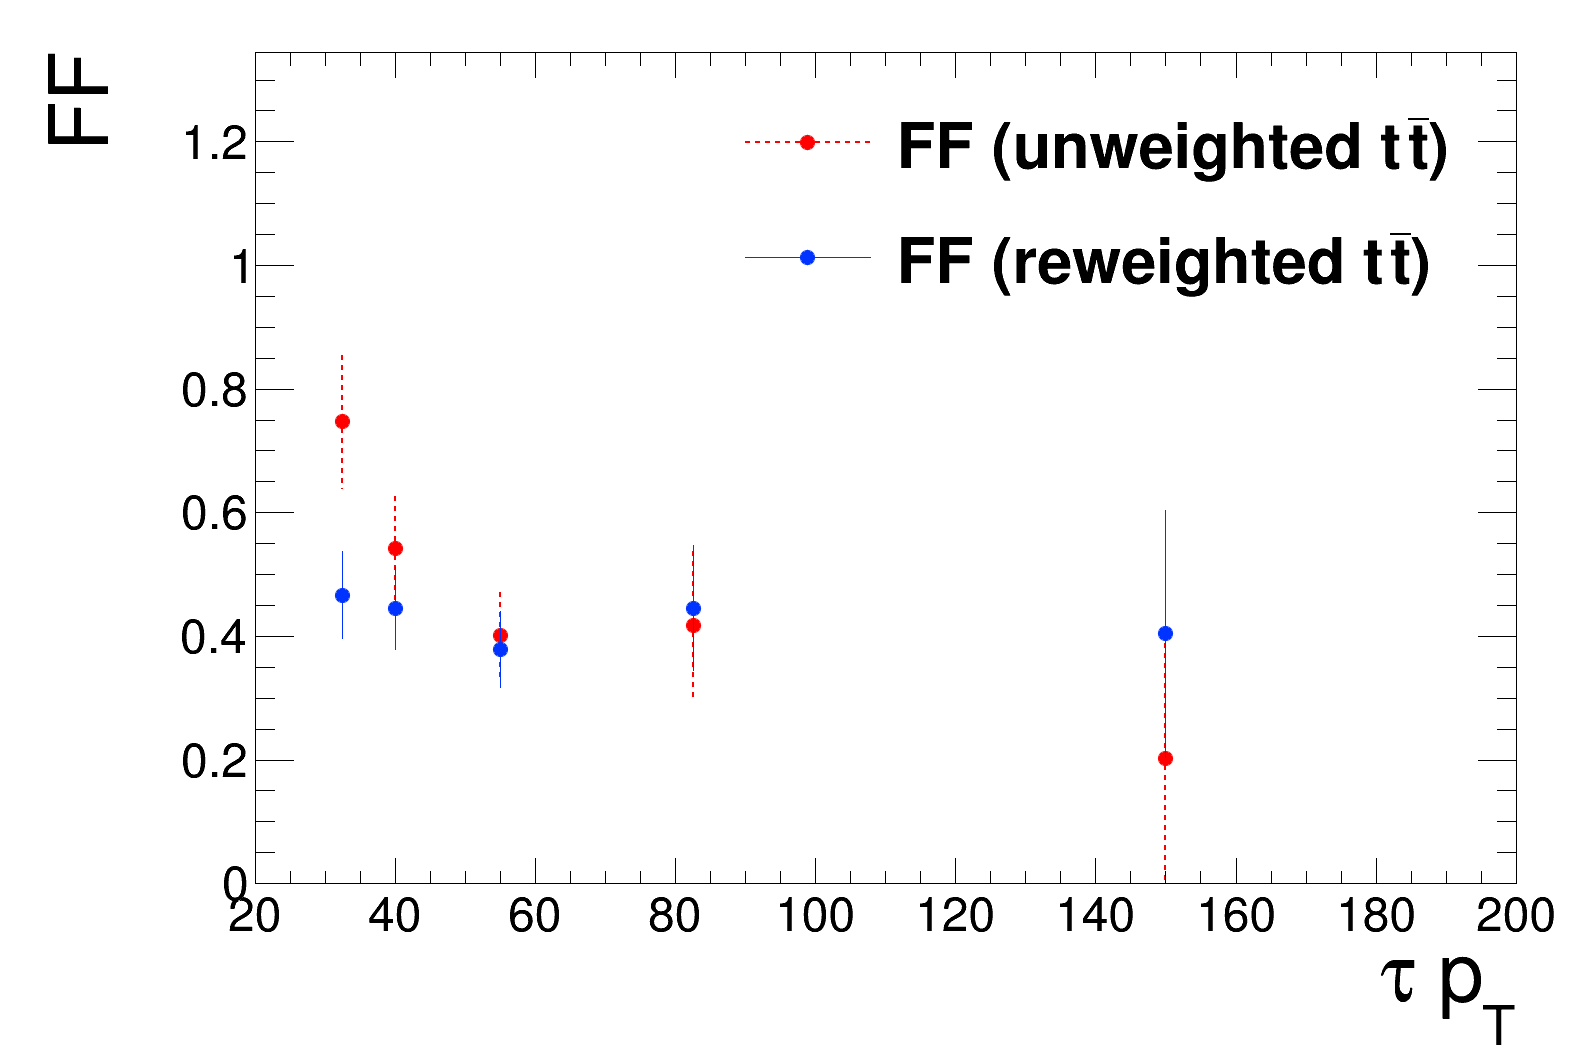
\includegraphics[width=.4\textwidth]{DiHiggs/plots/FF_CRs/LTTInvCR1p.png}
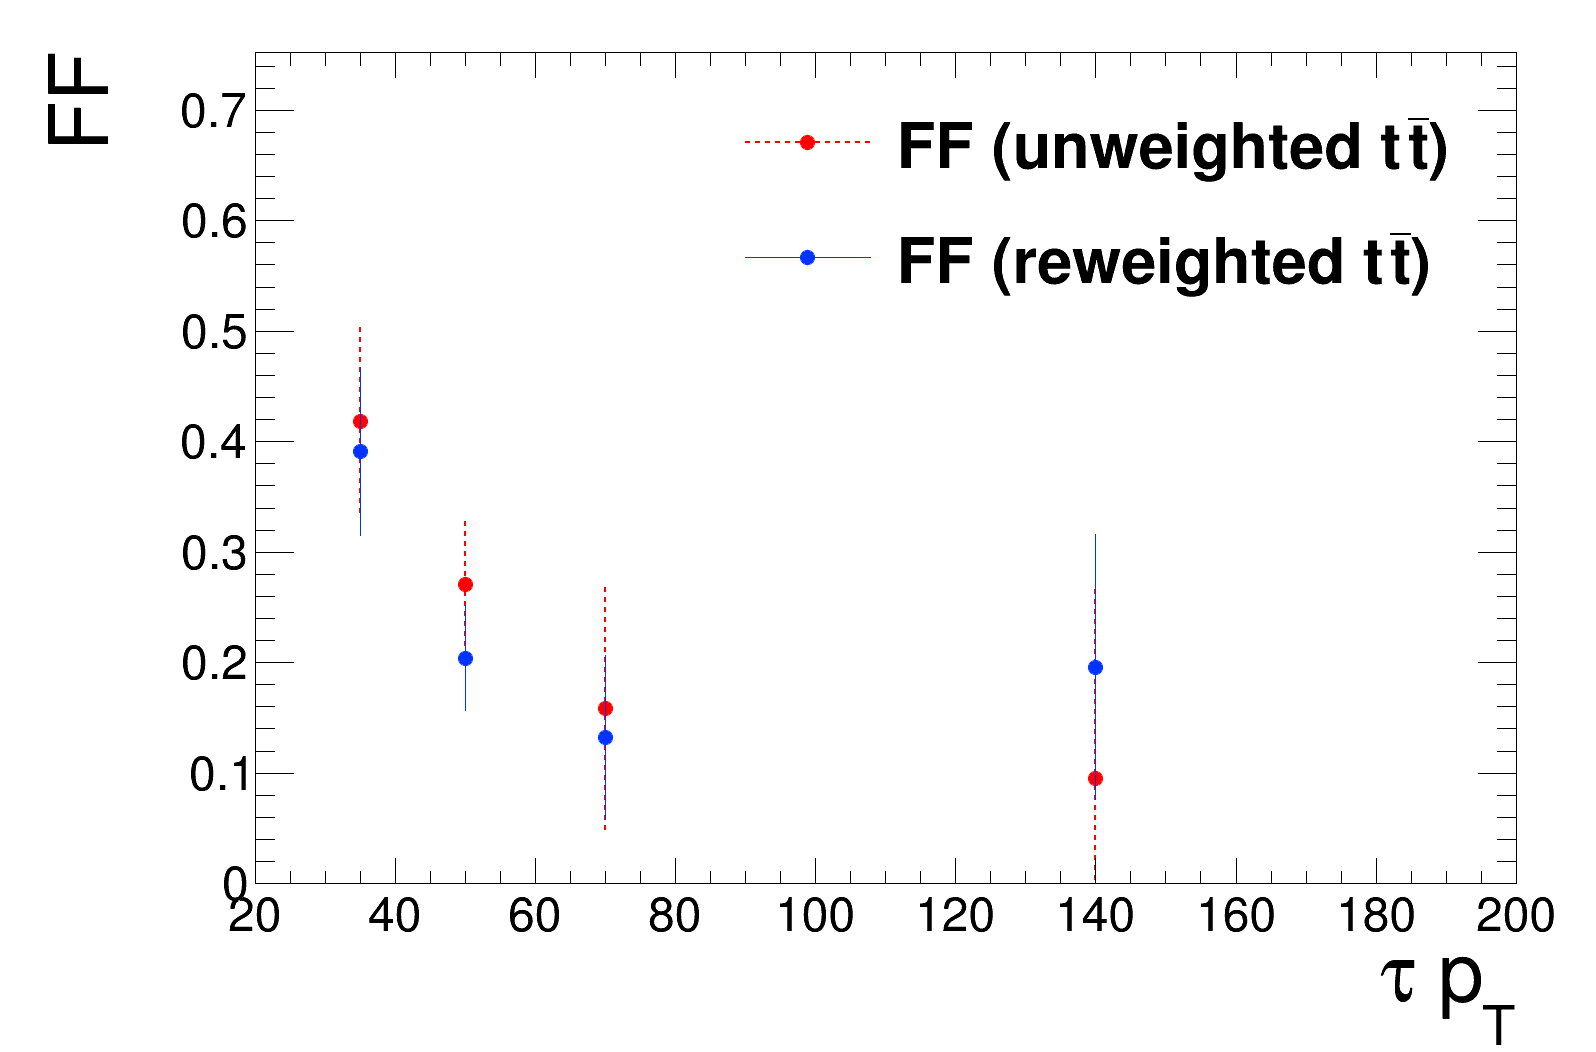
\includegraphics[width=.4\textwidth]{DiHiggs/plots/FF_CRs/LTTInvCR3p.png}\\
\caption{Fake factors for 1-prong (left) and 3-prong (right) \tauhad\ candidates for \ttbar\ processes (top) and multi-jet (bottom) for the \lephad LTT category.}
\label{fig:LTT_FF}
\end{figure}

\begin{figure}[htbp]
\centering
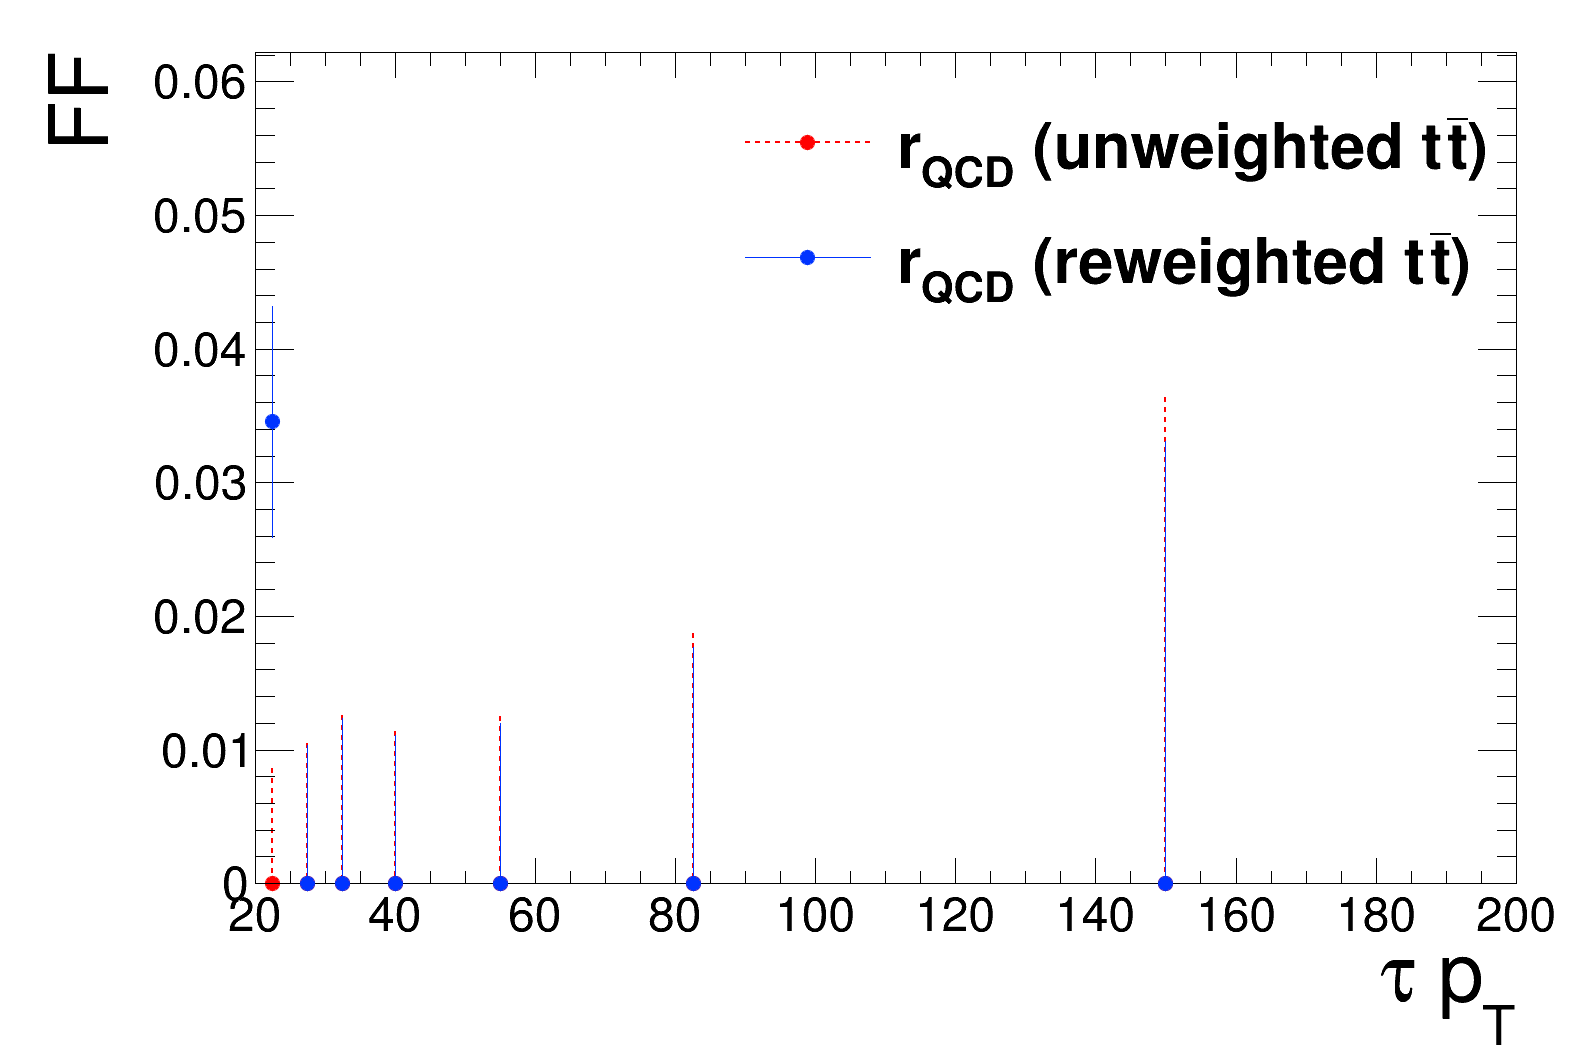
\includegraphics[width=.4\textwidth]{DiHiggs/plots/FF_CRs/SLTElecrQCD1p.png}
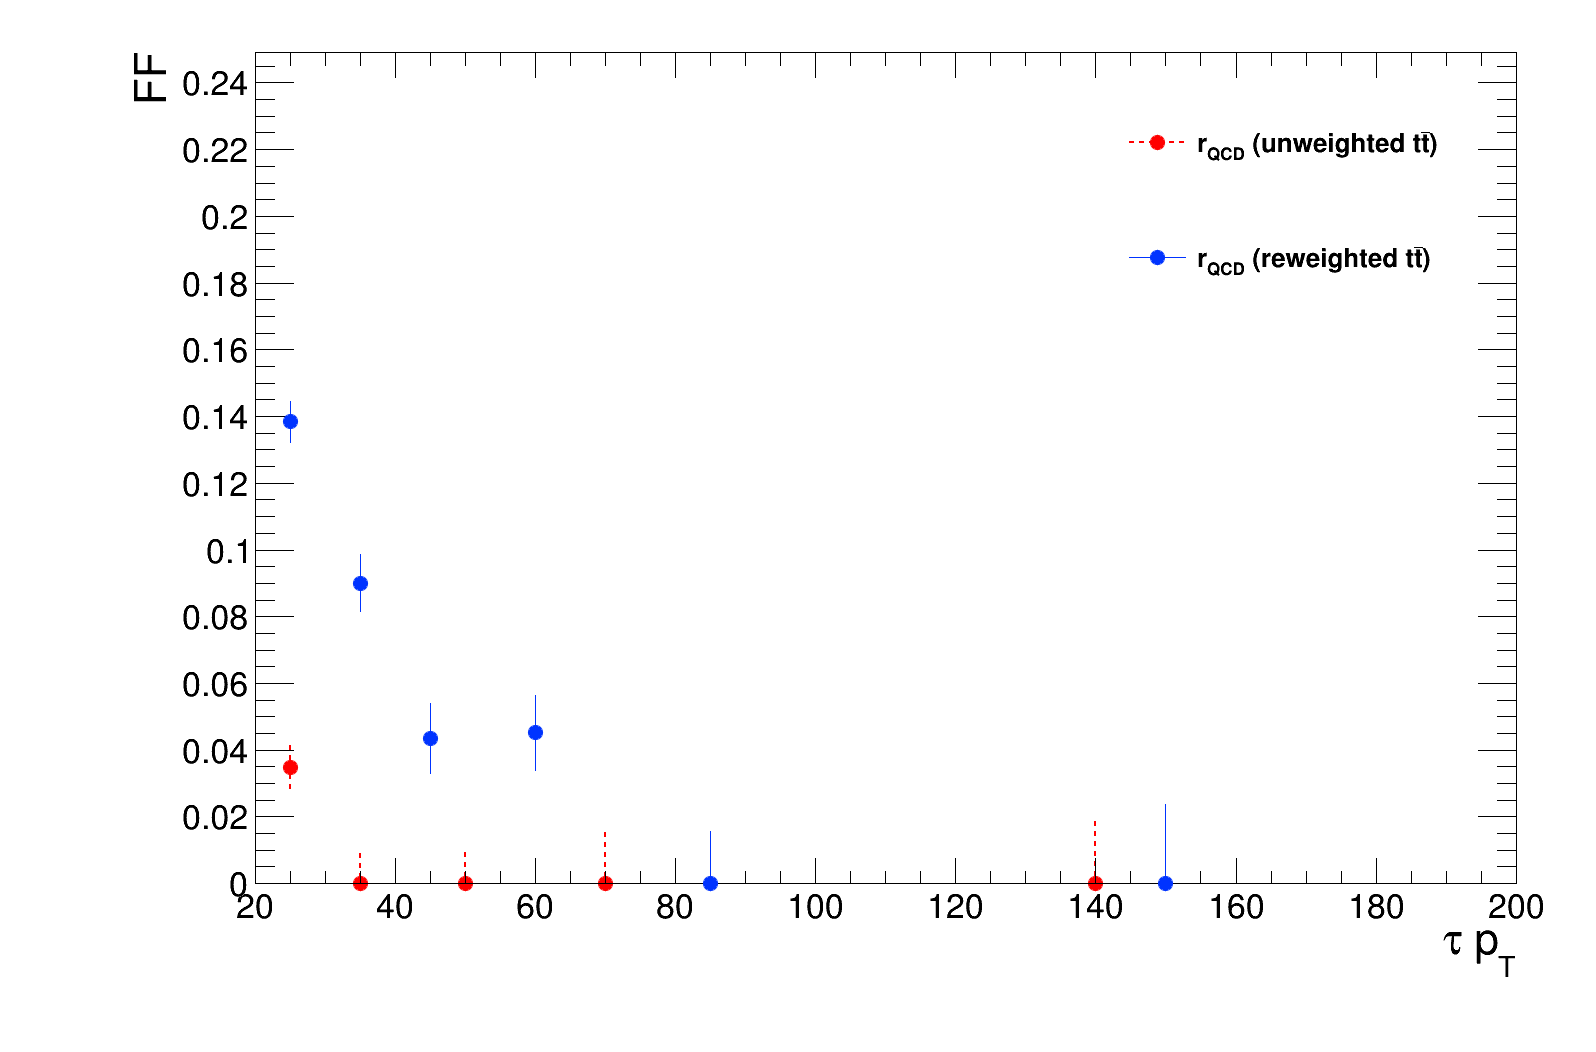
\includegraphics[width=.4\textwidth]{DiHiggs/plots/FF_CRs/SLTElecrQCD3p.png} \\
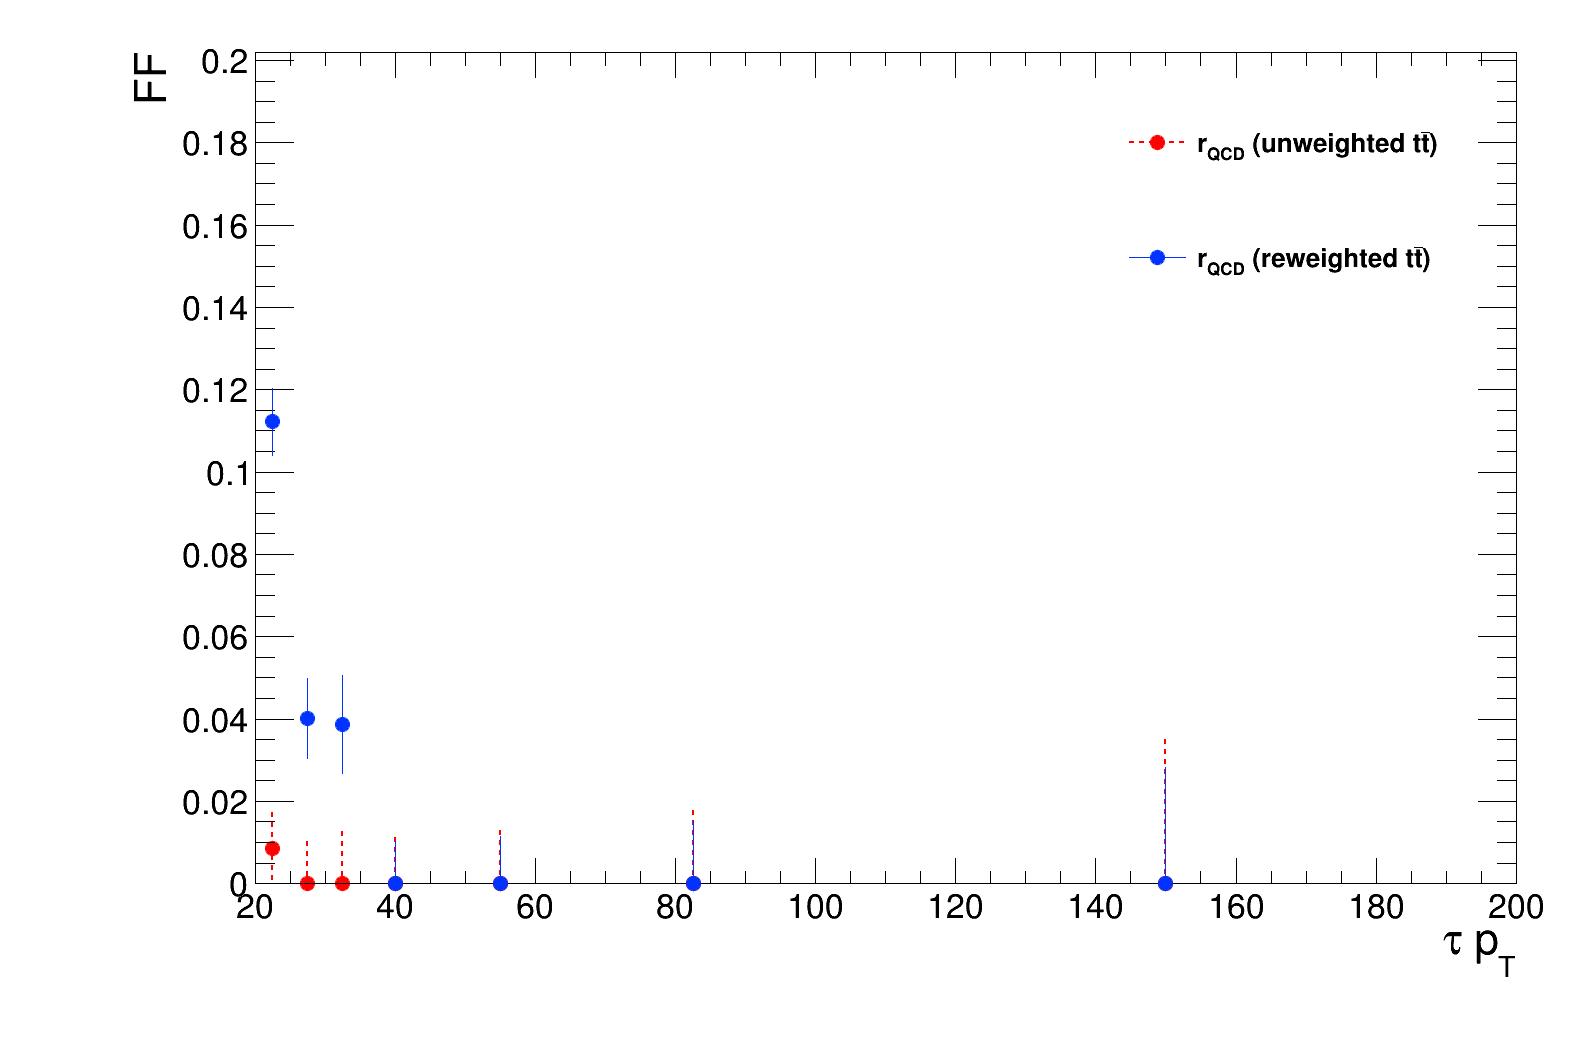
\includegraphics[width=.4\textwidth]{DiHiggs/plots/FF_CRs/SLTMuonrQCD1p.png}
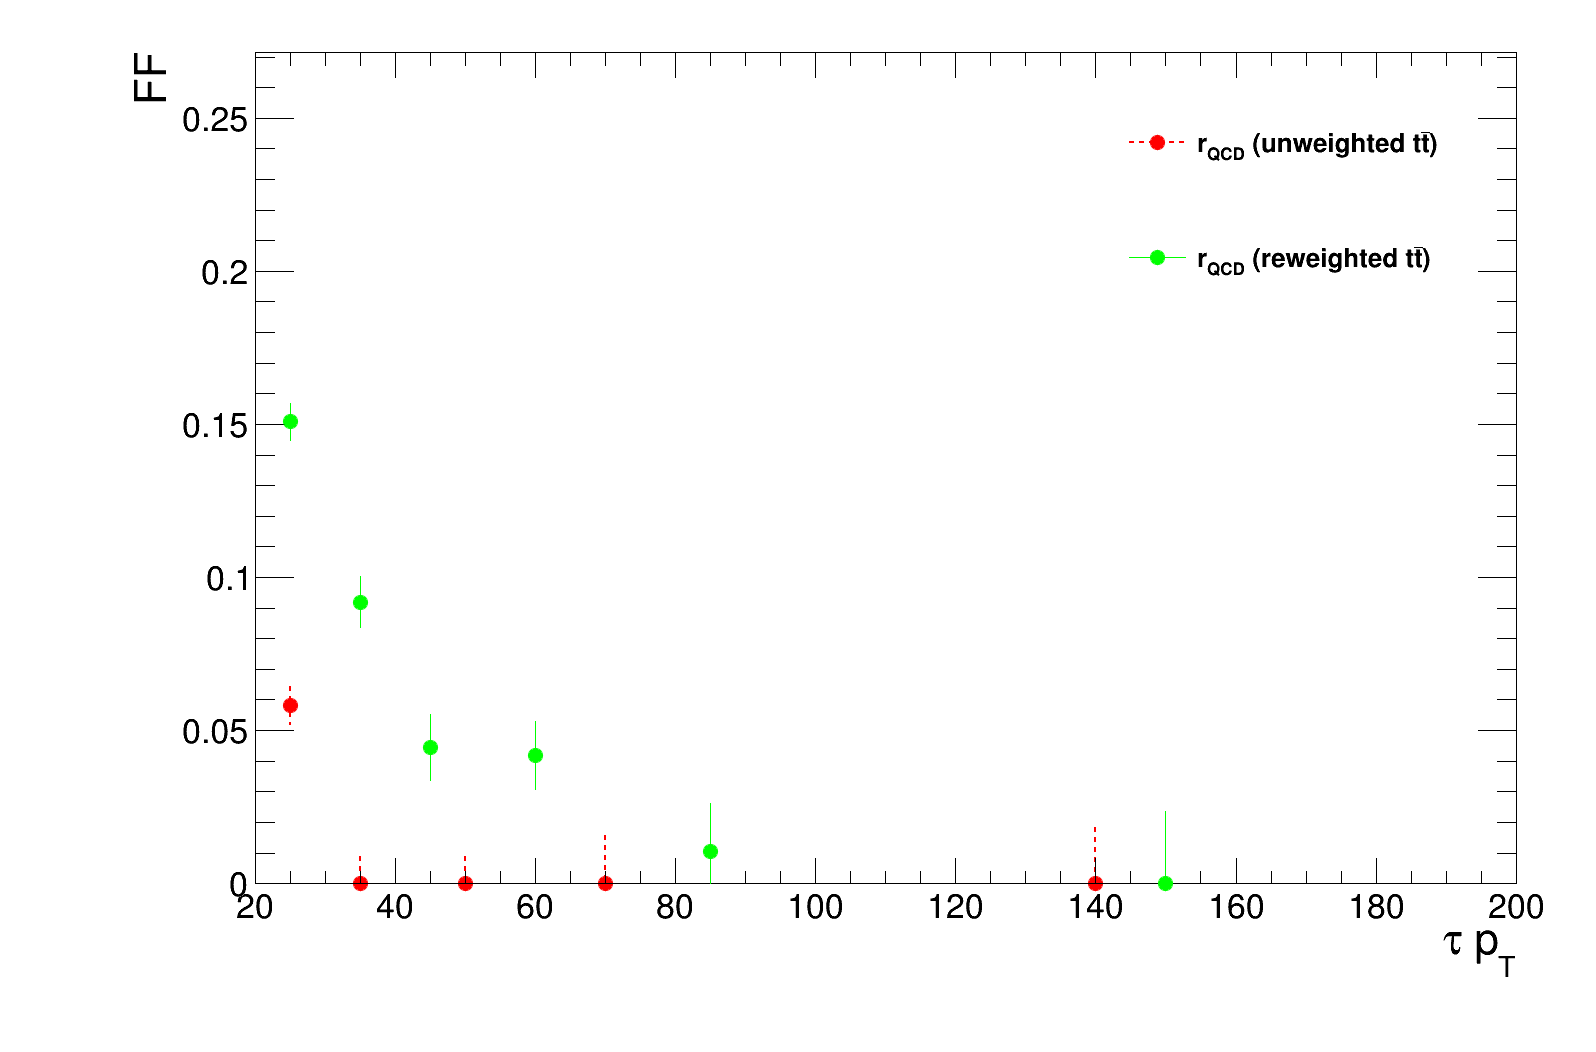
\includegraphics[width=.4\textwidth]{DiHiggs/plots/FF_CRs/SLTMuonrQCD3p.png}\\
\caption{$\mathrm{r}_{\mathrm{QCD}}$ for 1-prong (left) and 3-prong (right) \tauhad\ candidates for $e\tauhad$ channel (top) and $\mu\tauhad$ (bottom)
for the SLT channel.}
\label{fig:SLT_rQCD}
\end{figure}

\begin{figure}[htbp]
\centering
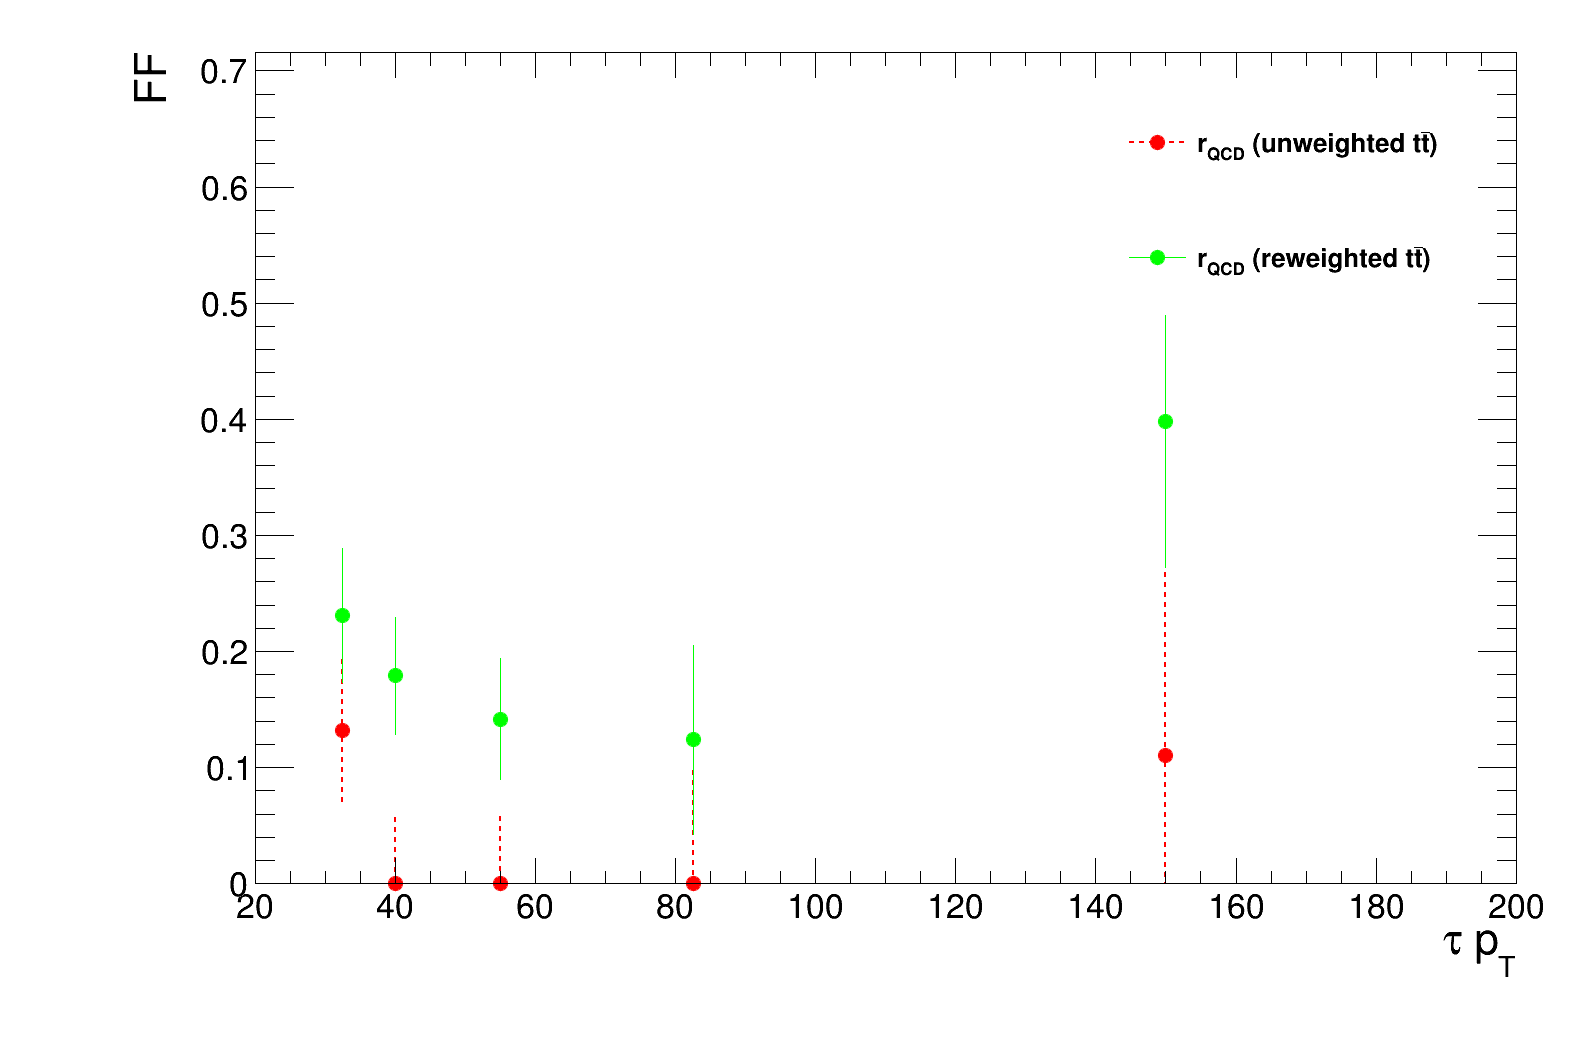
\includegraphics[width=.4\textwidth]{DiHiggs/plots/FF_CRs/LTTElecrQCD1p.png}
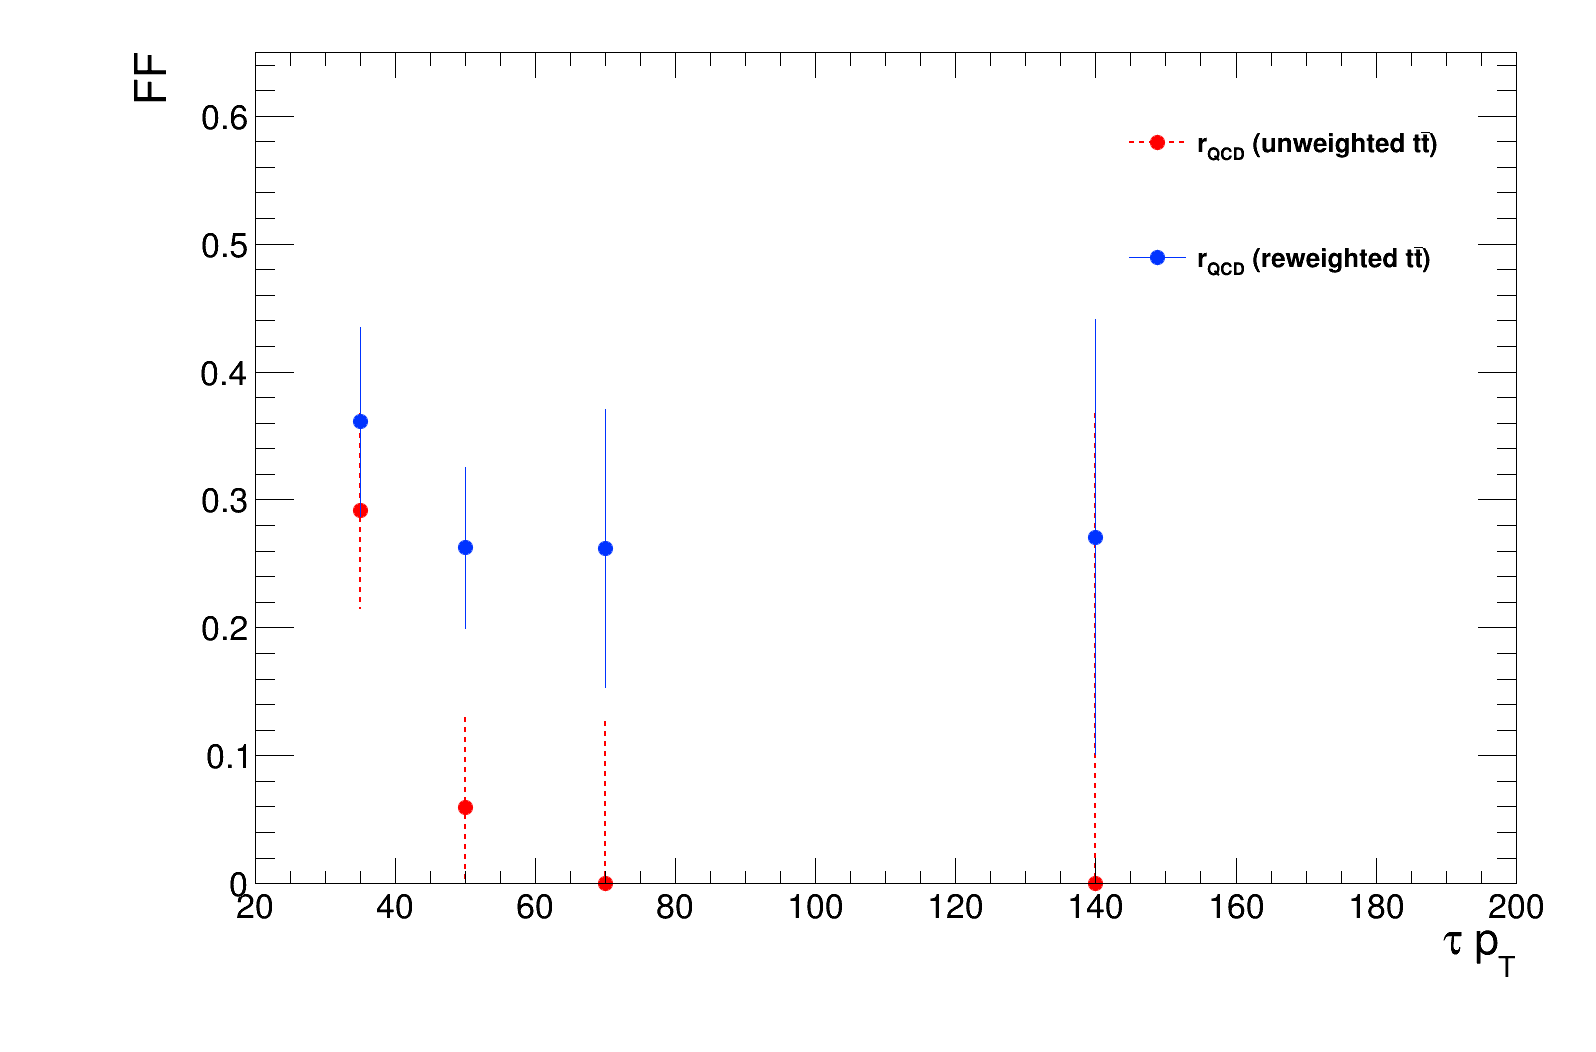
\includegraphics[width=.4\textwidth]{DiHiggs/plots/FF_CRs/LTTElecrQCD3p.png} \\
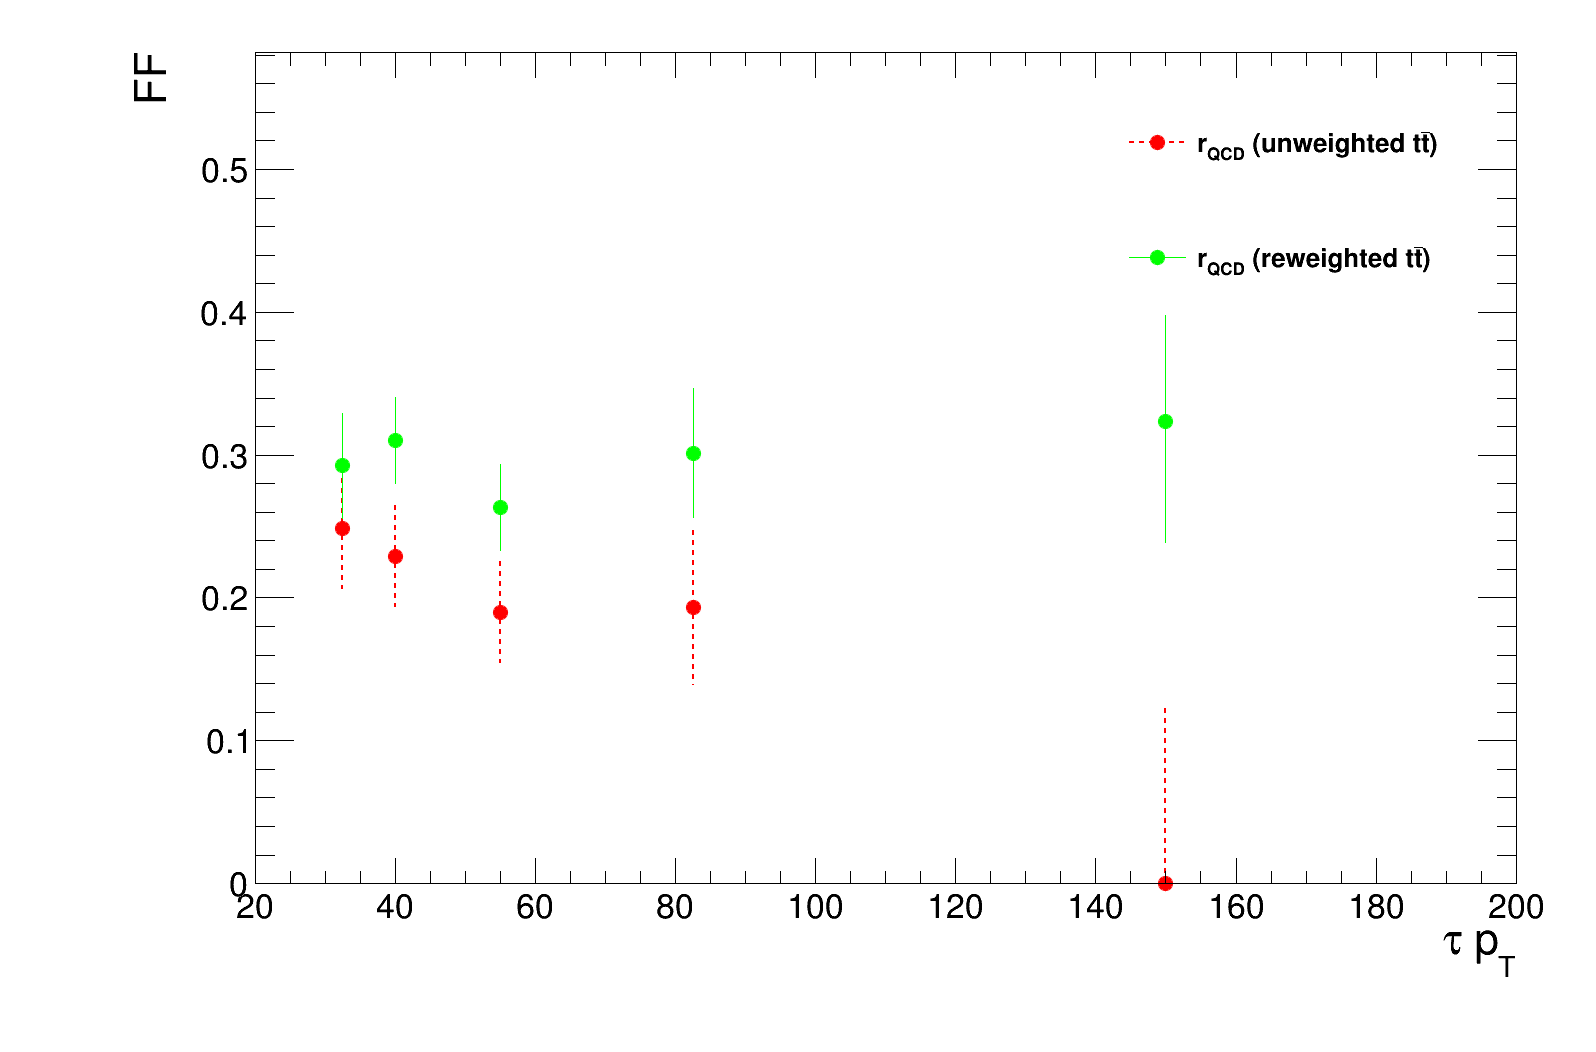
\includegraphics[width=.4\textwidth]{DiHiggs/plots/FF_CRs/LTTMuonrQCD1p.png}
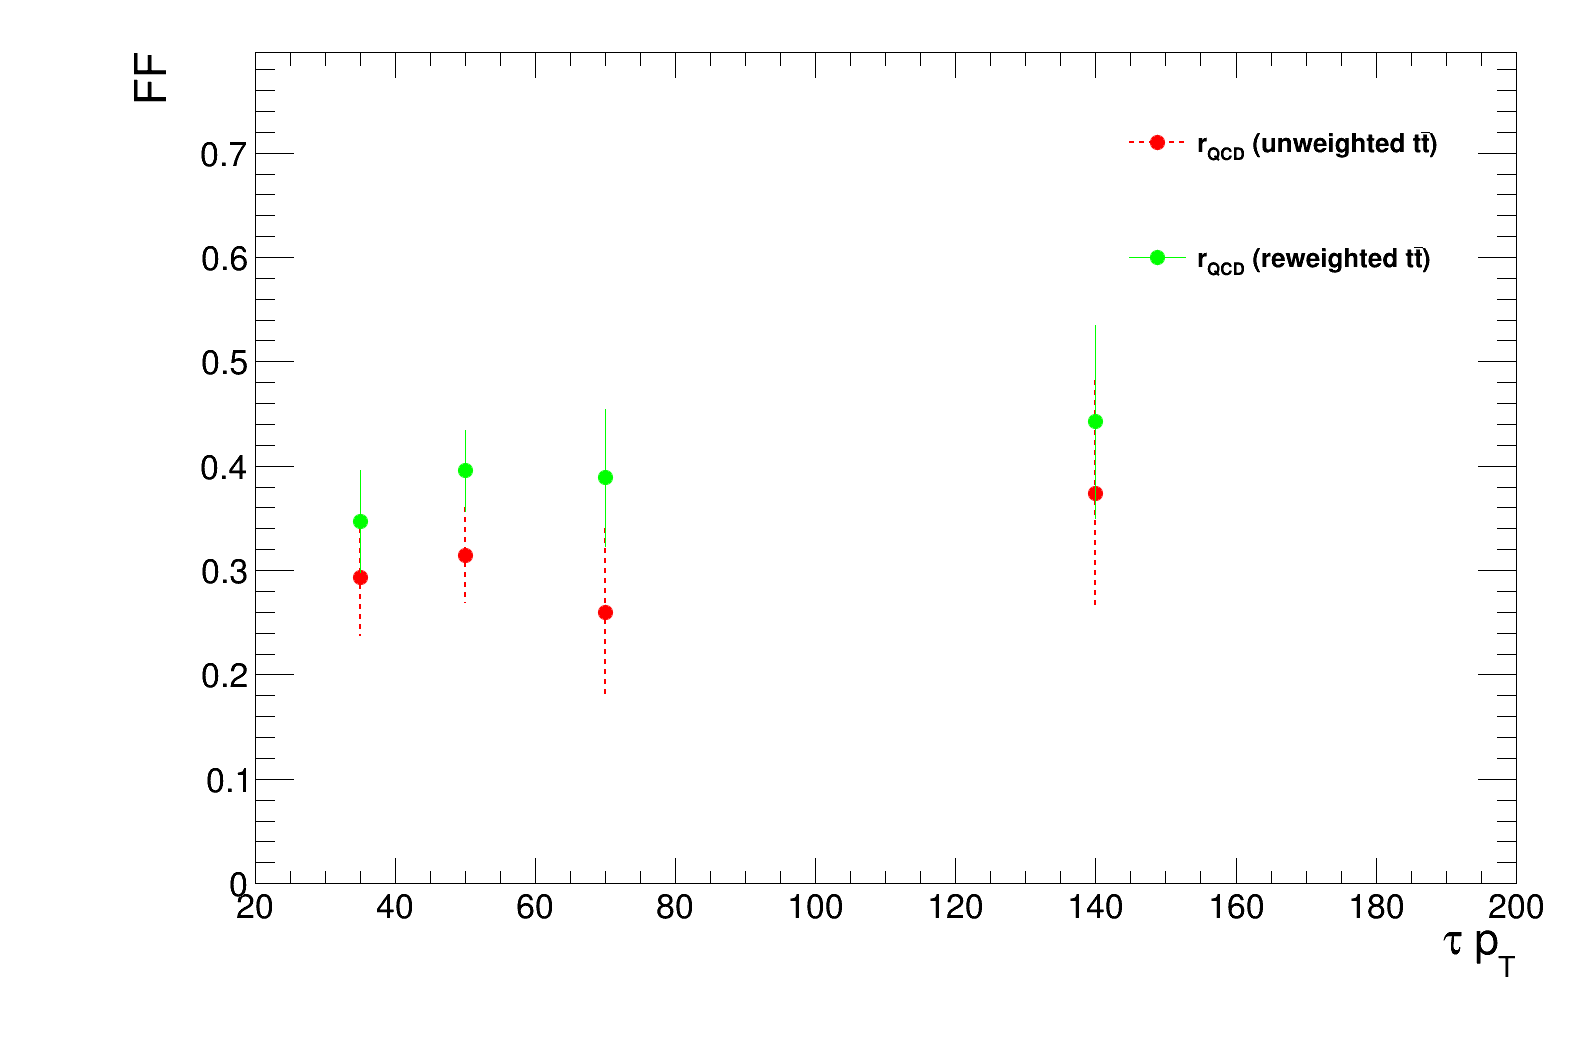
\includegraphics[width=.4\textwidth]{DiHiggs/plots/FF_CRs/LTTMuonrQCD3p.png}\\
\caption{$\mathrm{r}_{\mathrm{QCD}}$ for 1-prong (left) and 3-prong (right) \tauhad\ candidates for $e\tauhad$ channel (top) and $\mu\tauhad$ (bottom)
LTT channel.}
\label{fig:LTT_rQCD}
\end{figure}
%%%
% The difference between the fake-\tauhad\ background estimations obtained with and without
% the aforementioned $t\bar{t}$ modelling correction is taken as an uncertainty in the background estimate.
% A conservative 30\% modelling uncertainty is assigned to simulated non-$t\bar t$ backgrounds
% which are subtracted from data.
%%%The value of $\mathrm{r}_\text{multi-jet}$ is allowed to vary within $\pm 0.5$ with respect to the nominal estimate
%%%in the signal extraction fit to account for uncertainties in the modelling of the simulation used in its calculation.
% Due to its large dependence on the modelling of simulated $t\bar{t}$ events with fake-\tauhad\ 
% the obtained values of $\mathrm{r}_\text{multi-jet}$ are varied by $\pm 0.5$, while enforcing $0\leq r_\text{QCD}\leq 1$. 
% The impact of such a conservative uncertainty is small since the FFs in multi-jet and $t\bar{t}$ events are found to be similar.
%%%
% The total uncertainty on the $\text{FF}_\text{comb}$ for the SLT category is up to 10\% and
% up to 25\% for the LTT category.
%%%
The combined FF method is validated in
the 0-$b$-tagged and 1-$b$-tagged regions, where the same event selection as SR 
is applied but with different numbers of $b$-tagged jets required. 
The fakes in each validation region are estimated with FF calculated in each validation region 
with the same method used in the 2-$b$-tagged region.
These two validation regions are chosen as 
the signal contamination in the 0-$b$-tagged 
and 1-$b$-tagged regions is negligible,
and the 0-$b$-tagged region can benefit from its rich statistics 
and the 1-$b$-tagged region can benefit from being closer to the SR.
The estimated background distributions agree well 
with the observed distributions in all validation regions.
The data and MC comparison with fakes estimated with the FF method 
are shown in Figure~\ref{fig:FFVRSLT} for the SLT channel and
Figure~\ref{fig:FFVRLTT} for the LTT channel. 

\begin{figure}[htbp]
\centering
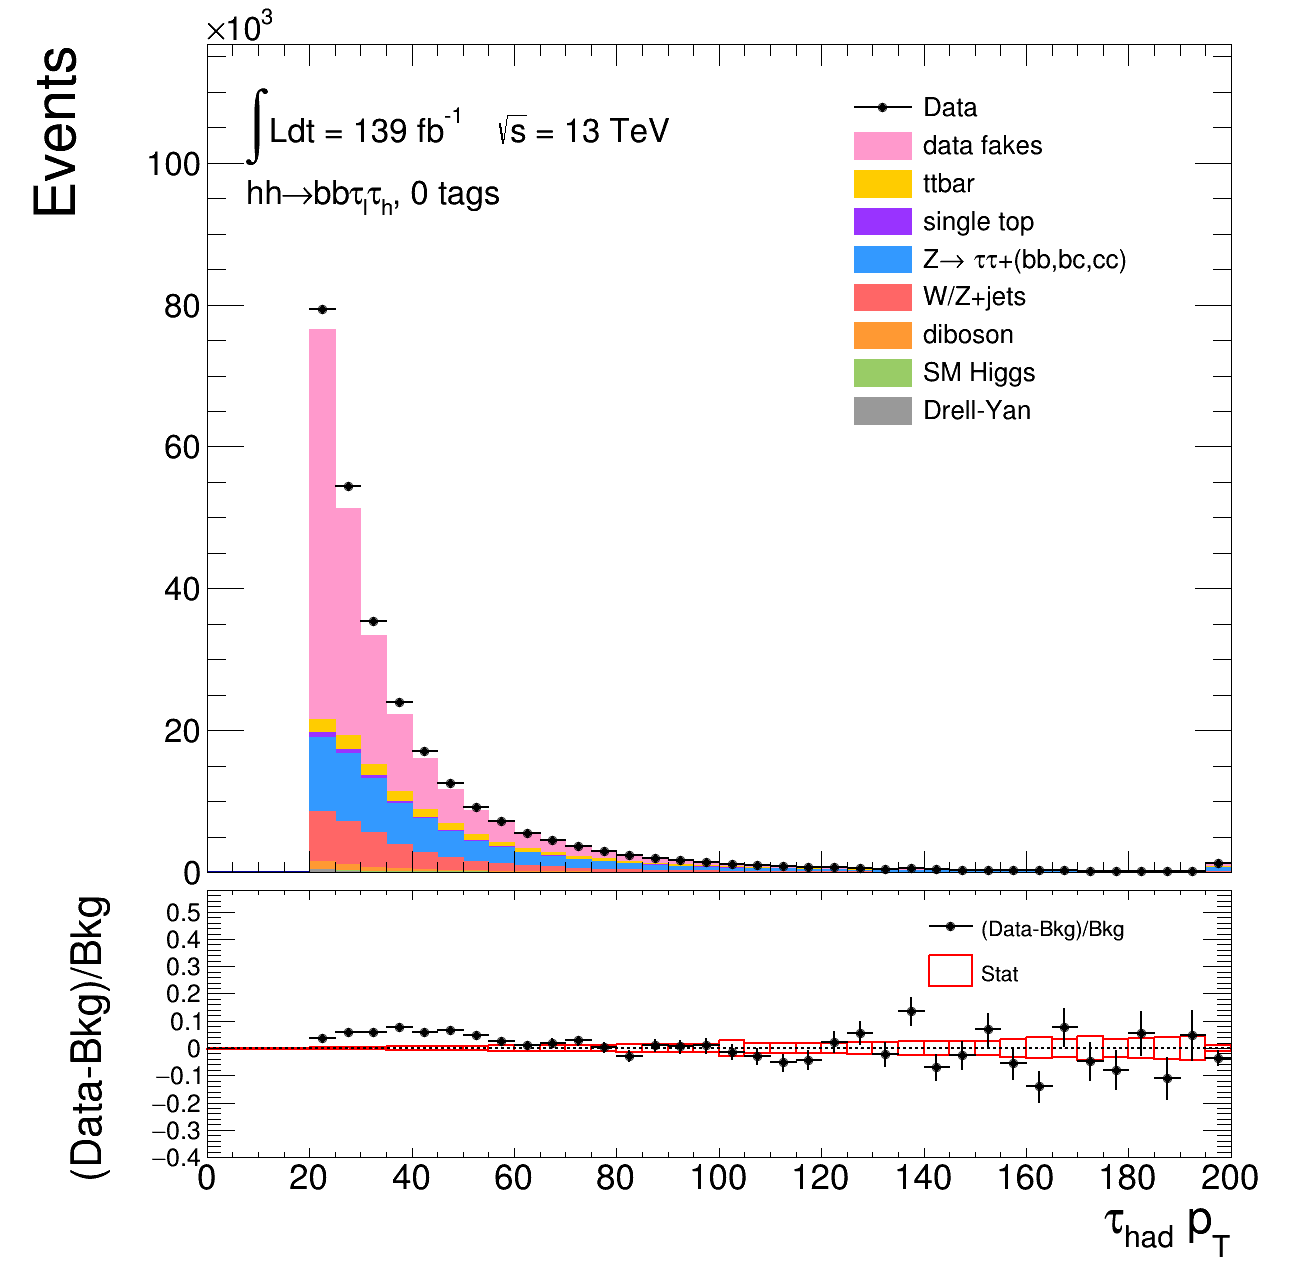
\includegraphics[width=.4\textwidth]{DiHiggs/plots/FF_CRs/SR_SLT_datafakes/HNone/BDTVarsHighMbb/0/C_0tag2pjet_0ptv_TauPt.png}
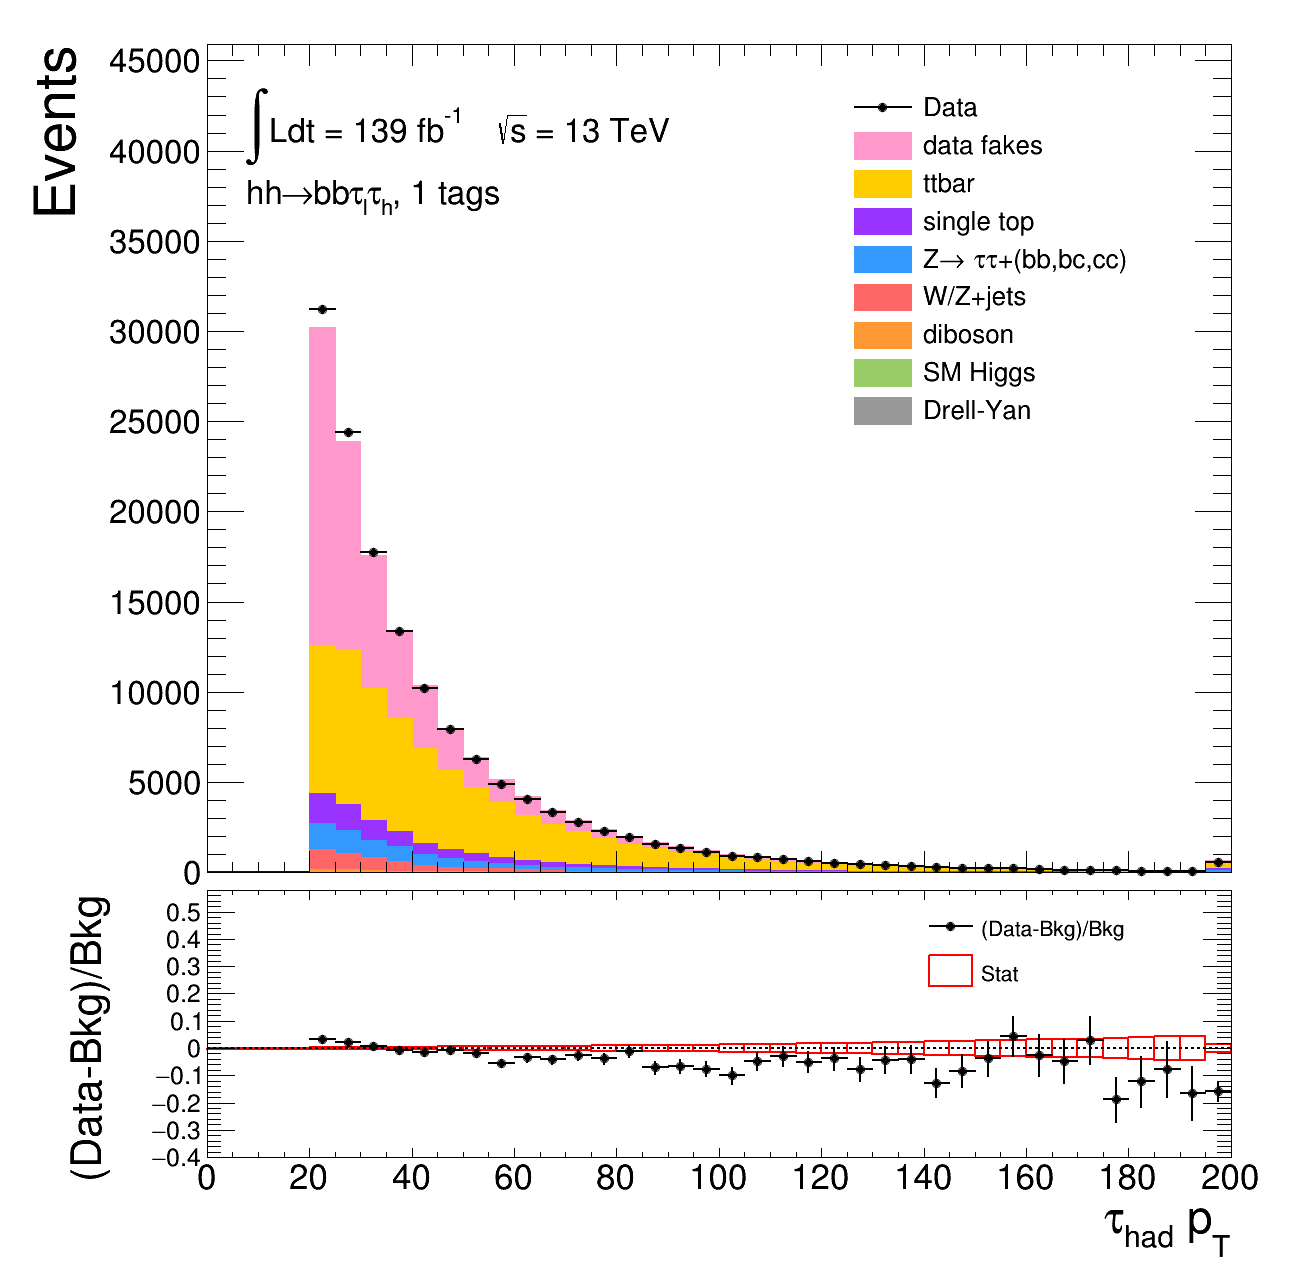
\includegraphics[width=.4\textwidth]{DiHiggs/plots/FF_CRs/SR_SLT_datafakes/HNone/BDTVarsHighMbb/1/C_1tag2pjet_0ptv_TauPt.png} \\
\caption{A comparison of data and background with fakes estimated with combined FF evaluated at the 0-$b$-tagged (left) 
and 1-$b$-tagged region (right) for the SLT channel. }
\label{fig:FFVRSLT}
\end{figure}


\begin{figure}[htbp]
\centering
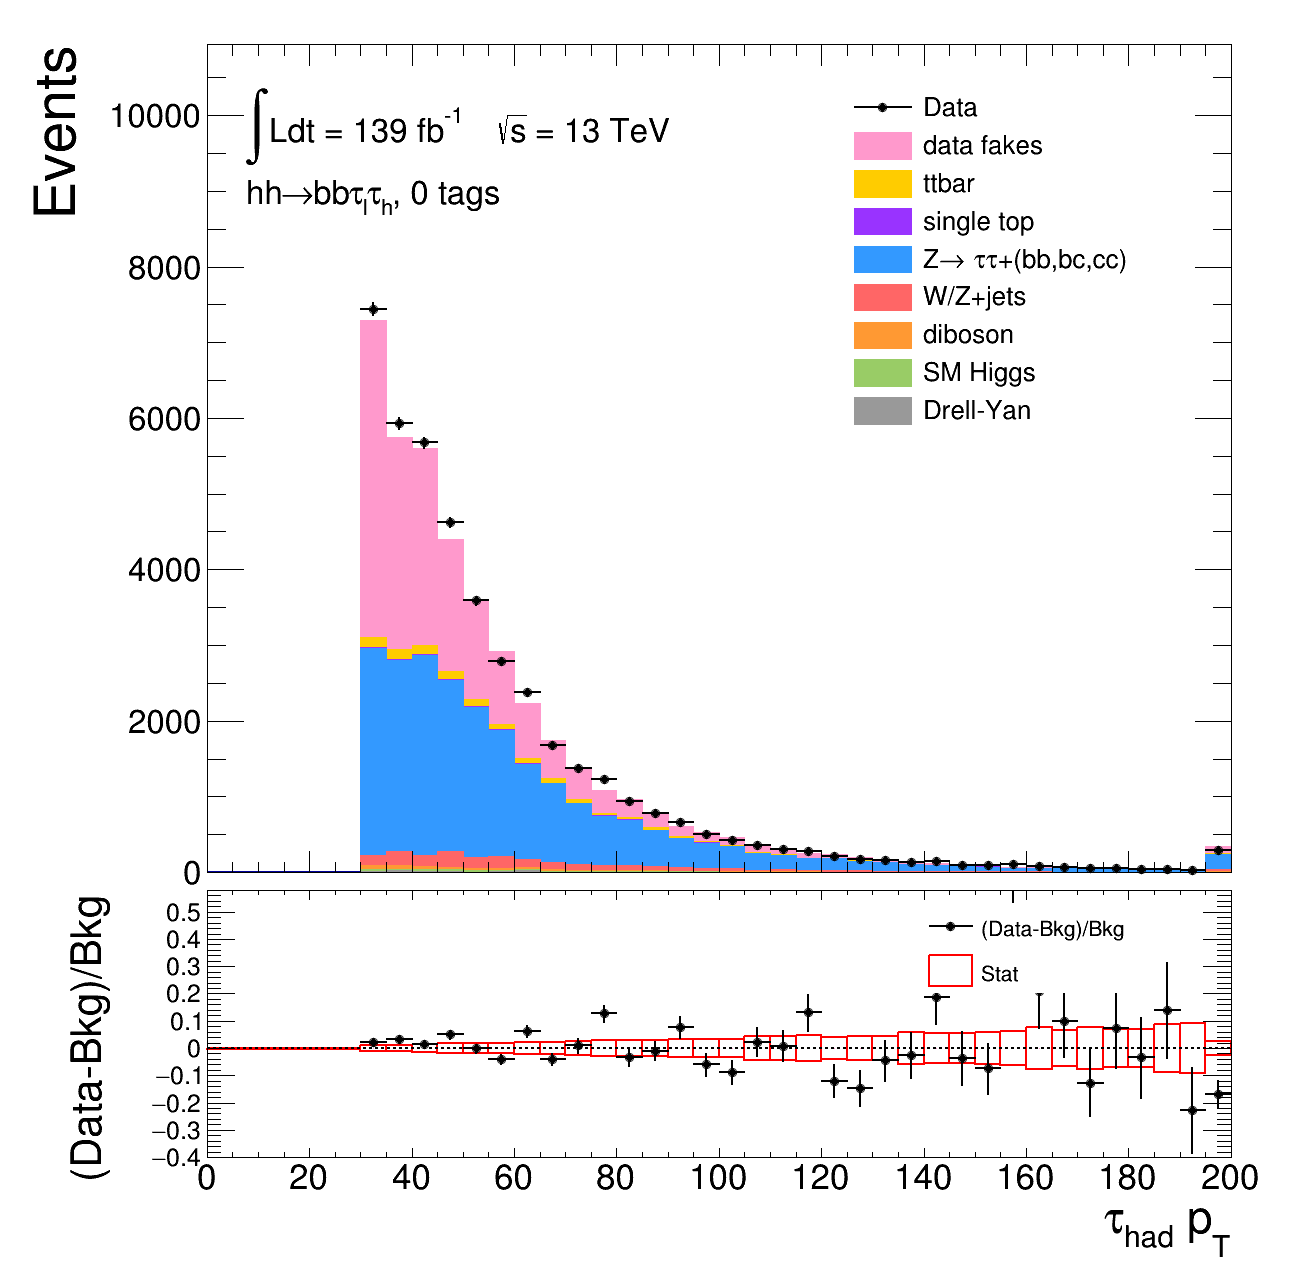
\includegraphics[width=.4\textwidth]{DiHiggs/plots/FF_CRs/SR_LTT_datafakes/HNone/BDTVarsHighMbb/0/C_0tag2pjet_0ptv_TauPt.png}
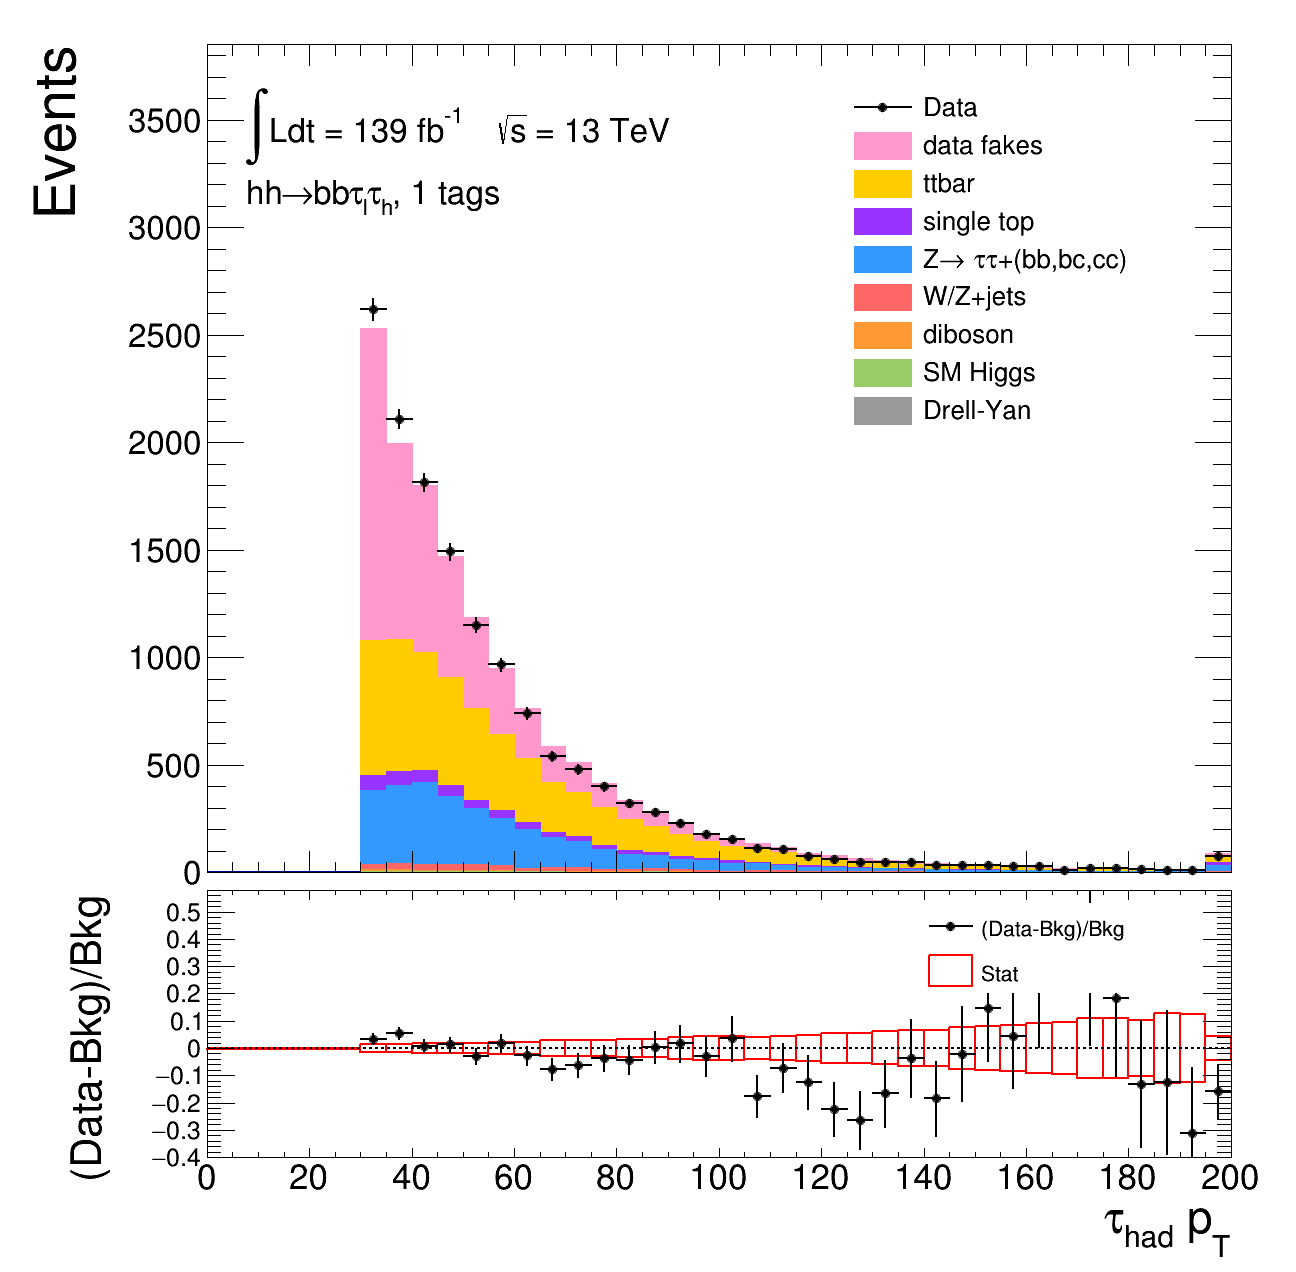
\includegraphics[width=.4\textwidth]{DiHiggs/plots/FF_CRs/SR_LTT_datafakes/HNone/BDTVarsHighMbb/1/C_1tag2pjet_0ptv_TauPt.png} \\
\caption{A comparison of data and background with fakes estimated with combined FF evaluated at the 0-$b$-tagged (left) 
and 1-$b$-tagged region (right) for the LTT channel. }
\label{fig:FFVRLTT}
\end{figure}









